\documentclass[12pt,letterpaper]{article}
% --- KHAI BÁO THƯ VIỆN ---
\usepackage[T1]{fontenc}
\usepackage{lmodern}
\usepackage{amsmath}
\usepackage[vietnamese]{babel}
\usepackage{graphicx}
\usepackage{mystyle}
\usepackage{float} 
\usepackage{xltabular}
\usepackage{tikz}
\usetikzlibrary{shapes.multipart} % Dùng để chia hộp node thành 3 phần (tên lớp, thuộc tính, phương thức)
\usetikzlibrary{arrows.meta}
\usepackage{enumitem}
\usepackage{dirtree}
\usetikzlibrary{shapes.geometric} % Để vẽ hình elip (ellipse) trong sơ đồ khối
\usetikzlibrary{positioning}      % Để căn chỉnh vị trí tương đối (below=of, right=of)
\tcbuselibrary{minted, breakable} % Bắt buộc phải có breakable ở đây
% --- Thư viện chèn và tô màu Code (C++) ---
\usepackage{minted}               % Lõi tô màu code
\usepackage{tcolorbox}            % Vẽ hộp màu bo góc bao quanh code
\tcbuselibrary{minted}            % Lệnh bắt buộc để trộn tcolorbox và minted vào nhau

% Căn lề để chữ không bị đè vào họa tiết ở góc
\geometry{
    left=2.5cm,
    right=2.5cm,
    top=3cm,
    bottom=3cm
}

% Cài đặt màu chủ đạo cho họa tiết (Màu xanh đậm)
\definecolor{titlepagecolor}{cmyk}{1,.60,0,.40}

% --- CODE VẼ ĐỒ HOẠ TRANG BÌA ---
\newcommand\titlepagedecoration{%
\begin{tikzpicture}[remember picture,overlay,shorten >= -10pt]

\coordinate (aux1) at ([yshift=-15pt]current page.north east);
\coordinate (aux2) at ([yshift=-410pt]current page.north east);
\coordinate (aux3) at ([xshift=-4.5cm]current page.north east);
\coordinate (aux4) at ([yshift=-150pt]current page.north east);

\begin{scope}[titlepagecolor!40,line width=12pt,rounded corners=12pt]
\draw
  (aux1) -- coordinate (a)
  ++(225:5) --
  ++(-45:5.1) coordinate (b);
\draw[shorten <= -10pt]
  (aux3) --
  (a) --
  (aux1);
\draw[opacity=0.6,titlepagecolor,shorten <= -10pt]
  (b) --
  ++(225:2.2) --
  ++(-45:2.2);
\end{scope}
\draw[titlepagecolor,line width=8pt,rounded corners=8pt,shorten <= -10pt]
  (aux4) --
  ++(225:0.8) --
  ++(-45:0.8);
\begin{scope}[titlepagecolor!70,line width=6pt,rounded corners=8pt]
\draw[shorten <= -10pt]
  (aux2) --
  ++(225:3) coordinate[pos=0.45] (c) --
  ++(-45:3.1);
\draw
  (aux2) --
  (c) --
  ++(135:2.5) --
  ++(45:2.5) --
  ++(-45:2.5) coordinate[pos=0.3] (d);   
\draw 
  (d) -- +(45:1);
\end{scope}
\end{tikzpicture}%
}

\begin{document}
\begin{titlepage}

% Gọi hàm vẽ các đường cong trang trí ở góc
\titlepagedecoration 

% --- PHẦN 1: LOGO VÀ TÊN TRƯỜNG ---
\begin{center}
    \begin{tabular}{c c c}
        % Đổi 'logo_hust.png' và 'logo_fami.png' thành ảnh của bạn đã tải lên Overleaf
        \raisebox{-0.5\height}{
\includegraphics[height=3cm]{hust_logo.png}} & 
        \begin{tabular}{c}
            \textcolor{titlepagecolor}{\textbf{\large ĐẠI HỌC BÁCH KHOA HÀ NỘI}} \\
            \textcolor{titlepagecolor}{\textbf{\large KHOA TOÁN - TIN}}
        \end{tabular} & 
        \raisebox{-0.5\height}{
\includegraphics[height=3cm]{fami_logo.png}}
    \end{tabular}
\end{center}

\vspace{0.8cm}

% --- PHẦN 2: TÊN MÔN HỌC ---
\noindent\textcolor{titlepagecolor}{\rule{\textwidth}{1pt}}
\vspace{0.cm}

\begin{center}
    \textcolor{titlepagecolor}{\Large \textbf{Báo cáo môn học}} \\[0.3cm]
    \textcolor{titlepagecolor}{\huge \textbf{KỸ THUẬT LẬP TRÌNH}}
\end{center}

\vspace{0.2cm}
\noindent\textcolor{titlepagecolor}{\rule{\textwidth}{1pt}}

\vspace{0.cm}

% --- PHẦN 3: TÊN ĐỀ TÀI ---
\begin{center}
    \textcolor{titlepagecolor}{\Huge \textbf{Chủ đề:}} \\[0.6cm]
    \textcolor{titlepagecolor}{\huge \textbf{Quản lý chi tiêu cá nhân}}
\end{center}
\vspace{0.5cm}
% --- PHẦN 4: THÔNG TIN NHÓM THỰC HIỆN ---

\vfill 

\begin{center}
    \large
    \renewcommand{\arraystretch}{1.3} % Giãn dòng cho thoáng
    % Đã tăng độ rộng cột 1 lên 6.5cm để chữ không bị rớt dòng
    \begin{tabular}{@{}p{6.5cm} l l@{}}
        \textbf{Giảng viên hướng dẫn:} & \textbf{TS. Vũ Thành Nam} & \\[0.2cm]
        \textbf{Nhóm số 69:}& Hứa Ngọc Khánh              & \textbf{202419070} \\
                                       & Phạm Thị Ninh               & \textbf{202419086} \\[0.2cm] 
        \textbf{Mã lớp:}               & \textbf{169313}               & \\
    \end{tabular}
\end{center}


% --- PHẦN 5: ĐỊA ĐIỂM, THỜI GIAN ---

\begin{center}
    \vfill
    \large \textbf{Hà Nội, 6/2026}
\end{center}

\vspace{1cm}

\end{titlepage}
\newpage
\tableofcontents
%------------------- NỘI DUNG BÁO CÁO BẮT ĐẦU TỪ ĐÂY---------------------------

\newpage
\section{Lời mở đầu}
Lời đầu tiên, chúng em xin gửi lời cảm ơn sâu sắc đến thầy Vũ Thành Nam. Sự giảng dạy, hỗ trợ và tạo điều kiện của thầy đã giúp chúng em hoàn thành tốt nhất báo cáo này. Chúc thầy có thật nhiều sức khỏe để tiếp tục công tác giảng dạy và nghiên cứu khoa học trong thời gian tới! 

Trong cuộc sống hiện đại, việc quản lý tài chính cá nhân ngày càng trở nên quan trọng. Tuy nhiên, nhiều người vẫn gặp khó khăn trong việc theo dõi các khoản thu nhập, chi tiêu cũng như kiểm soát ngân sách của bản thân. Việc ghi chép thủ công bằng sổ sách hoặc bảng tính thường mất nhiều thời gian, dễ sai sót và khó tổng hợp khi khối lượng dữ liệu ngày càng lớn.

Xuất phát từ nhu cầu đó, nhóm đã xây dựng hệ thống \textbf{Quản lý chi tiêu cá nhân} nhằm hỗ trợ người dùng lưu trữ, theo dõi và thống kê các khoản thu chi một cách thuận tiện. Hệ thống cho phép quản lý giao dịch, thiết lập ngân sách theo từng danh mục, cảnh báo khi vượt hạn mức chi tiêu và tạo các báo cáo trực quan giúp người dùng đánh giá tình hình tài chính của mình.

Thông qua đề tài này, nhóm không chỉ vận dụng các kiến thức về lập trình hướng đối tượng, cấu trúc dữ liệu và giải thuật đã học mà còn có cơ hội tiếp cận quy trình thiết kế và xây dựng một hệ thống phần mềm hoàn chỉnh, từ phân tích yêu cầu, thiết kế kiến trúc đến triển khai và kiểm thử hệ thống.
\setcounter{page}{1}

\newpage
\section{Phân tích  bài toán}
\subsection{Giới thiệu bài toán}
\subsubsection{Bối cảnh và vấn đề}

\begin{itemize}
\item Nhu cầu quản lý tài chính cá nhân ngày càng trở nên cần thiết trong cuộc sống hiện đại.

\item Các khoản thu và chi phát sinh liên tục theo thời gian, tạo ra khối lượng lớn dữ liệu giao dịch.

\item Người dùng thường gặp khó khăn trong việc:
\begin{itemize}
    \item Theo dõi các khoản thu chi.
    \item Kiểm soát ngân sách theo từng danh mục.
    \item Đánh giá tình hình tài chính cá nhân.
    \item Tổng hợp số liệu để lập báo cáo.
\end{itemize}

\item Các phương pháp quản lý truyền thống như sổ tay hoặc Excel có nhiều hạn chế:
\begin{itemize}
    \item Dễ thất lạc hoặc sai sót dữ liệu.
    \item Khó thống kê khi số lượng giao dịch lớn.
    \item Hạn chế khả năng kiểm soát ngân sách.
\end{itemize}

\item Khi số lượng giao dịch tăng lên, hệ thống cần có khả năng:
\begin{itemize}
    \item Lưu trữ dữ liệu hiệu quả.
    \item Tìm kiếm và thống kê nhanh.
    \item Hỗ trợ tạo báo cáo theo nhiều khoảng thời gian khác nhau.
\end{itemize}

\end{itemize}

\subsubsection{Mục tiêu hệ thống}

\begin{itemize}
\item Xây dựng hệ thống quản lý chi tiêu cá nhân có giao diện trực quan và dễ sử dụng.

\item Hỗ trợ người dùng:
\begin{itemize}
    \item Đăng ký và đăng nhập tài khoản.
    \item Quản lý thông tin cá nhân.
\end{itemize}

\item Thiết lập ngân sách cho từng danh mục chi tiêu theo tháng.
\item Cho phép ghi nhận và quản lý các giao dịch:
\begin{itemize}
    \item Giao dịch thu.
    \item Giao dịch chi.
    \item Lưu trữ lịch sử giao dịch.
\end{itemize}

\item Tự động cập nhật ngân sách sau mỗi giao dịch phát sinh.

\item Cảnh báo khi mức chi tiêu vượt quá ngân sách đã thiết lập.

\item Hỗ trợ trực quan thống kê và báo cáo theo từng khoảng thời gian tùy chọn

\item Trực quan hóa dữ liệu bằng biểu đồ và cung cấp nhận xét hỗ trợ người dùng đánh giá tình hình tài chính.

\item Vận dụng các cấu trúc dữ liệu và thuật toán đã học để tổ chức, quản lý và xử lý dữ liệu trong hệ thống.
\end{itemize}
\subsection{Phân tích bài toán}

Bài toán đặt ra là xây dựng một hệ thống quản lý chi tiêu cá nhân bằng ngôn ngữ Python, sử dụng thư viện Tkinter để xây dựng giao diện người dùng và Matplotlib để trực quan hóa dữ liệu. Hệ thống cho phép người dùng quản lý các khoản thu, chi, thiết lập ngân sách và theo dõi tình hình tài chính cá nhân thông qua các báo cáo thống kê trực quan.

Dữ liệu của hệ thống phải được lưu trữ bền vững để đảm bảo khả năng khôi phục sau khi chương trình được khởi động lại. Đồng thời, hệ thống cần hỗ trợ các chức năng tìm kiếm, thống kê, cảnh báo vượt ngân sách và tạo báo cáo theo nhiều khoảng thời gian khác nhau.

\textbf{Input}

\begin{itemize}
\item \textbf{Dữ liệu nhập từ giao diện người dùng}
\begin{itemize}
\item Thông tin đăng ký và đăng nhập tài khoản.
\item Thông tin giao dịch thu, chi.
\item Thông tin ngân sách theo từng danh mục.
\item Thông tin danh mục chi tiêu và thu nhập.
\end{itemize}
\item \textbf{Dữ liệu đọc từ file JSON}
\begin{itemize}
    \item users.json
    \item transactions.json
    \item budgets.json
    \item categories.json
    \item reports.json
\end{itemize}

\item Các dữ liệu đọc từ file được chuyển đổi thành các đối tượng và cấu trúc dữ liệu tương ứng trong bộ nhớ để phục vụ xử lý.

\end{itemize}

\textbf{Output}

\begin{itemize}
\item \textbf{Lịch sử giao dịch}
\begin{itemize}
\item Hiển thị danh sách các khoản thu và chi.
\item Hỗ trợ tra cứu và xóa giao dịch.
\end{itemize}
\item \textbf{Cảnh báo ngân sách}
\begin{itemize}
    \item Phát hiện các danh mục vượt ngân sách.
    \item Hiển thị thông báo cảnh báo cho người dùng.
\end{itemize}

\item \textbf{Báo cáo thống kê}
\begin{itemize}
    \item Tổng hợp thu nhập và chi tiêu.
    \item Tính toán số dư hiện tại.
    \item Thống kê chi tiêu theo từng danh mục.
    \item Tính tỷ lệ chi tiêu của từng danh mục.
\end{itemize}

\item \textbf{Biểu đồ trực quan}
\begin{itemize}
    \item Biểu đồ tỷ lệ chi tiêu theo danh mục.
    \item Biểu đồ được xây dựng bằng thư viện Matplotlib.
\end{itemize}

\item \textbf{Kết quả phân tích tài chính}
\begin{itemize}
    \item Tổng thu.
    \item Tổng chi.
    \item Số dư còn lại.
    \item Các danh mục vượt ngân sách.
\end{itemize}
\end{itemize}
\newpage
\section{Thiết kế chương trình}
\subsection{Tổng thể chức năng}
\begin{itemize}
    \item \textbf{Quản lý Giao dịch (Transaction)}
    \begin{itemize}
        \item \textbf{Ghi chép giao dịch mới}: Hệ thống cho phép người dùng thêm khoản thu/chi thực tế. 
        \begin{itemize}
            \item Số tiền phải là số thực dương lớn hơn 0.
            \item Danh sách danh mục hiển thị trong Dropdown (\texttt{Combobox}) tự động thay đổi dựa trên Loại giao dịch (Thu/Chi) mà người dùng thao tác chọn trước đó.
            \item Ngay sau khi thêm thành công một giao dịch thuộc loại Chi tiêu, hệ thống tự động kiểm tra ngân sách của danh mục tương ứng.
        \end{itemize}
        \item \textbf{Xóa giao dịch}: Cho phép xóa hoàn toàn khoản chi tiêu/thu nhập đã nhập sai thông qua ID. Mọi thao tác xóa giao dịch chi đều làm cập nhật lại tổng chi thực tế của danh mục, ảnh hưởng trực tiếp đến trạng thái cảnh báo của Ngân sách.
        \item \textbf{Xem lịch sử giao dịch}: Lịch sử được hiển thị dưới dạng bảng. Cho phép người dùng lọc nhanh danh sách theo khoảng thời gian (Từ ngày - Đến ngày) và theo Loại giao dịch (Tất cả / Thu nhập / Chi tiêu).
    \end{itemize}
    \item \textbf{Quản lý Ngân sách (Budget)}
    \begin{itemize}
        \item \textbf{Đặt hạn mức ngân sách}: Cho phép thiết lập số tiền tối đa được phép chi tiêu cho một danh mục trong một tháng cụ thể.
        \begin{itemize}
            \item Mỗi danh mục chi chỉ được phép có duy nhất 01 ngân sách trong cùng một tháng. Nếu đã tồn tại, hệ thống tự động chuyển sang chế độ ghi đè cập nhật hạn mức mới.
            \item Hạn mức ngân sách phải là số thực dương.
        \end{itemize}
        \item \textbf{Kiểm tra và Cảnh báo vượt mức}: Hệ thống liên tục so sánh tổng số tiền chi thực tế của danh mục với hạn mức đã đặt. Nếu số tiền chi vượt qua hạn mức ngân sách, hệ thống kích hoạt cảnh báo trực quan trên giao diện (đổi màu thanh tiến trình sang màu đỏ và xuất hiện popup cảnh báo rủi ro) để báo động cho người dùng.
    \end{itemize}
    \item \textbf{Báo cáo và Thống kê (Report)}
    \begin{itemize}
        \item \textbf{Tổng hợp số liệu kỳ}: Tự động quét và tính toán dữ liệu trong khoảng thời gian tùy chọn (ngày, tuần, tháng, năm).
        \begin{itemize}
            \item Tính tổng thu (\texttt{totalIncome}) và tổng chi (\texttt{totalExpense}).
            \item Tính toán Số dư hiện tại (\texttt{Balance = totalIncome - totalExpense}) và hiển thị tổng quan.
            \item Tính tổng số tiền đã chi chi tiết theo từng danh mục và quy ra tỉ lệ phần trăm tương ứng.
        \end{itemize}
        \item \textbf{Xuất báo cáo đồ họa}: Trích xuất dữ liệu từ \texttt{categorySummaries} và sử dụng thư viện \texttt{Matplotlib} để kết xuất biểu đồ đồ họa. Dùng biểu đồ tròn (Pie chart) để thể hiện rõ nét tỷ trọng chi tiêu giữa các nhóm danh mục.
    \end{itemize}
    \item \textbf{Quản lý lưu trữ dữ liệu}
    \begin{itemize}
        \item \textbf{Đọc dữ liệu từ file}: Khi khởi động ứng dụng, kiến trúc Repository tự động tải toàn bộ nội dung từ các file \texttt{users.json}, \texttt{categories.json}, \texttt{budgets.json}, \texttt{reports.json} và \texttt{transactions.json} vào bộ nhớ.
        \item \textbf{Ghi dữ liệu xuống file}: Sau mỗi thao tác (Thêm / Sửa / Xóa) làm thay đổi dữ liệu của thực thể, hệ thống tự động gọi phương thức \texttt{\_save\_all()} của lớp \texttt{BaseRepository} để ghi đè trạng thái hiện tại của bộ nhớ xuống file vật lý.
        \begin{itemize}
            \item Đảm bảo tính bền vững của dữ liệu nếu chương trình bị đóng hoặc mất điện đột ngột.
            \item Cấu trúc JSON đảm bảo lưu trữ chuẩn xác mảng các đối tượng (objects) với đầy đủ key-value tương ứng theo thuộc tính lớp.
        \end{itemize}
    \end{itemize}
\end{itemize}
\subsection{Luồng nghiệp vụ hệ thống}

Hệ thống quản lý chi tiêu cá nhân được xây dựng nhằm hỗ trợ người dùng theo dõi các khoản thu, chi, quản lý ngân sách và tạo báo cáo tài chính. Luồng nghiệp vụ của hệ thống được mô tả như sau:

\begin{itemize}

\item \textbf{Đăng ký tài khoản}
\begin{itemize}
\item Người dùng nhập địa chỉ email và mật khẩu.
\item Hệ thống kiểm tra tính hợp lệ của email và mật khẩu.
\item Nếu thông tin hợp lệ, tài khoản được lưu vào cơ sở dữ liệu.
\end{itemize}

\item \textbf{Đăng nhập hệ thống}
\begin{itemize}
\item Người dùng nhập email và mật khẩu đã đăng ký.
\item Hệ thống xác thực thông tin đăng nhập.
\item Nếu thông tin chính xác, người dùng được phép truy cập các chức năng của hệ thống.
\end{itemize}

\item \textbf{Thiết lập ngân sách}
\begin{itemize}
\item Người dùng tạo ngân sách theo từng tháng.
\item Người dùng thiết lập ngân sách cho từng danh mục chi tiêu.
\item Ngân sách được sử dụng để theo dõi và kiểm soát chi tiêu.
\end{itemize}

\item \textbf{Nhập giao dịch}
\begin{itemize}
\item Chọn ngày thực hiện giao dịch.
\item Chọn loại giao dịch (thu hoặc chi).
\item Nhập ghi chú (không bắt buộc).
\item Nhập số tiền giao dịch.
\item Chọn danh mục giao dịch.
\item Xác nhận lưu giao dịch.
\end{itemize}

\item \textbf{Cập nhật ngân sách và lưu trữ dữ liệu}
\begin{itemize}
\item Tự động cập nhật số tiền đã sử dụng của danh mục tương ứng.
\item Trừ ngân sách đối với các giao dịch chi tiêu (nếu danh mục đã được thiết lập ngân sách).
\item Lưu thông tin giao dịch vào cơ sở dữ liệu.
\item Cập nhật lịch sử giao dịch để phục vụ tra cứu và thống kê.
\end{itemize}

\item \textbf{Kiểm tra ngân sách và cảnh báo}
\begin{itemize}
\item Kiểm tra mức sử dụng ngân sách của từng danh mục.
\item Xác định các danh mục có chi tiêu vượt ngân sách.
\item Hiển thị cảnh báo để người dùng điều chỉnh kế hoạch chi tiêu.
\end{itemize}

\item \textbf{Tạo báo cáo tài chính}
\begin{itemize}
\item Cho phép lựa chọn khoảng thời gian báo cáo:
\begin{itemize}
\item Theo ngày.
\item Theo tuần.
\item Theo tháng.
\item Theo quý.
\item Theo năm.
\item Khoảng thời gian tùy chọn.
\end{itemize}
\item Tổng hợp các khoản thu, chi và tính toán số dư.
\item Phân loại giao dịch theo danh mục.
\item Tính tỷ lệ chi tiêu của từng danh mục.
\item Xác định các danh mục vượt ngân sách.

\end{itemize}

\item \textbf{Trực quan hóa dữ liệu và nhận xét}
\begin{itemize}
\item Tạo biểu đồ thể hiện tỷ lệ chi tiêu theo từng danh mục.
\item Hiển thị các thông tin thống kê trực quan.
\item Đưa ra nhận xét bằng văn bản về tình hình tài chính của người dùng.
\end{itemize}

\item \textbf{Đăng xuất}
\begin{itemize}
\item Kết thúc phiên làm việc hiện tại.
\item Xóa thông tin đăng nhập khỏi bộ nhớ tạm của ứng dụng.
\item Quay trở lại màn hình đăng nhập ban đầu.
\end{itemize}

\end{itemize}

\subsection{Đối tượng}
Để đảm bảo hệ thống Quản lý chi tiêu cá nhân hoạt động ổn định và đáp ứng đầy đủ các luồng nghiệp vụ cốt lõi, cơ sở dữ liệu được thiết kế và mô hình hóa thành 5 lớp đối tượng trung tâm: User (Người dùng), Category (Danh mục), Transaction (Giao dịch), Budget (Ngân sách) và Report (Báo cáo). Các đối tượng này có mối liên kết chặt chẽ với nhau theo mô hình quan hệ. Cấu trúc dữ liệu chi tiết của từng lớp đối tượng được trình bày lần lượt trong các bảng dưới đây:

\subsubsection{User}
\begin{center}
    \begin{tabular}{|l|l|p{8.5cm}|}
        \hline
        \textbf{Tên Thuộc Tính} & \textbf{Kiểu Dữ Liệu} & \textbf{Mô Tả Chức Năng} \\ \hline
        id & int & Mã định danh người dùng (Khóa chính) \\ \hline
        name & string & Họ và tên hiển thị của người dùng \\ \hline
        email & string & Địa chỉ email dùng để đăng ký/đăng nhập vào hệ thống \\ \hline
        password & string & Mật khẩu đăng nhập hệ thống \\ \hline
        currency & string & Đơn vị tiền tệ hiển thị mặc định (VD: VND, USD) \\ \hline
        created\_at & datetime & Thời gian tài khoản được tạo lập vào hệ thống \\ \hline
    \end{tabular}
    
    \vspace{0.2cm}
    \textit{Bảng 1: Cấu trúc dữ liệu của User}
\end{center}
\subsubsection{Category}

\begin{center}
    \begin{tabular}{|l|l|p{8.5cm}|}
        \hline
        \textbf{Tên Thuộc Tính} & \textbf{Kiểu Dữ Liệu} & \textbf{Mô Tả Chức Năng} \\ \hline
        id & int & Mã định danh danh mục (Khóa chính) \\ \hline
        name & string & Tên gọi của danh mục (VD: Ăn uống, Tiền nhà, Tiền lương) \\ \hline
        type & string & Phân loại danh mục thuộc nhóm Thu nhập hay Chi tiêu\\ \hline
    \end{tabular}
    
    \vspace{0.2cm}
    \textit{Bảng 2: Cấu trúc dữ liệu của Category}
\end{center}

\subsubsection{Transaction}

\begin{center}
    \begin{tabular}{|l|l|p{8.5cm}|}
        \hline
        \textbf{Tên Thuộc Tính} & \textbf{Kiểu Dữ Liệu} & \textbf{Mô Tả Chức Năng} \\ \hline
        id & int & Mã định danh giao dịch (Khóa chính) \\ \hline
        amount & decimal & Số tiền thu vào hoặc chi ra của giao dịch \\ \hline
        type & string & Phân loại luồng tiền (Thu hoặc Chi) \\ \hline
        note & string & Ghi chú, diễn giải thêm về mục đích của giao dịch (Tùy chọn) \\ \hline
        date & date & Ngày tháng năm thực hiện giao dịch thực tế \\ \hline
        created\_at & datetime & Dấu thời gian hệ thống ghi nhận bản ghi này \\ \hline
    \end{tabular}
    
    \vspace{0.2cm}
    \textit{Bảng 3: Cấu trúc dữ liệu của Transaction}
\end{center}
\subsubsection{Budget}
\begin{center}
    \begin{tabular}{|l|l|p{8.5cm}|}
        \hline
        \textbf{Tên Thuộc Tính} & \textbf{Kiểu Dữ Liệu} & \textbf{Mô Tả Chức Năng} \\ \hline
        id & int & Mã định danh ngân sách (Khóa chính) \\ \hline
        limit\_amount & decimal & Hạn mức số tiền tối đa được phép chi tiêu cho danh mục \\ \hline
        month & string & Tháng/Kỳ áp dụng hạn mức ngân sách này \\ \hline
        created\_at & datetime & Thời điểm bản ghi ngân sách được thiết lập \\ \hline
    \end{tabular}
    
    \vspace{0.2cm}
    \textit{Bảng 4: Cấu trúc dữ liệu của Budget}
\end{center}
\subsubsection{Report}
\begin{center}
 \begin{tabular}{|l|l|p{8.5cm}|}
        \hline
        \textbf{Thuộc tính} & \textbf{Kiểu dữ liệu} & \textbf{Mô tả} \\
        \hline
        id & int & Mã định danh duy nhất của báo cáo \\ \hline
        start\_date & string & Ngày bắt đầu kỳ báo cáo (YYYY-MM-DD) \\ \hline
        end\_date & string & Ngày kết thúc kỳ báo cáo (YYYY-MM-DD) \\ \hline
        period\_type & string & Loại kỳ (day, week, month, quarter, year, custom) \\ \hline
        total\_income & float & Tổng thu nhập trong kỳ \\ \hline
        total\_expense & float & Tổng chi tiêu trong kỳ \\ \hline
        balance & float & Số dư (total\_income - total\_expense) \\ \hline
        created\_at & string & Thời gian tạo báo cáo (YYYY-MM-DD HH:MM:SS) \\ \hline
        over\_budget\_categories & LinkedList & Danh sách các danh mục vượt hạn mức \\ \hline
        category\_summaries & LinkedList & Chi tiết thống kê danh mục (tên, chi, hạn mức, \%) \\ \hline
    \end{tabular}
    
    \vspace{0.2cm}
    \textit{Bảng 5: Cấu trúc dữ liệu của Report}
\end{center}

\newpage
\subsection{Mô hình thực thể liên kết (ERD)}
\begin{figure}[H]
    \centering
    \begin{tikzpicture}[
        scale=0.6, transform shape, 
        >=stealth,
        entity/.style={rectangle, draw=blue!70!black, thick, fill=blue!10, minimum width=2.8cm, minimum height=1.2cm, align=center, font=\bfseries},
        relationship/.style={diamond, draw=red!70!black, thick, fill=red!10, aspect=2, inner sep=2pt, minimum width=2.5cm, align=center, font=\small\bfseries},
        attribute/.style={ellipse, draw=purple!70!black, thick, fill=purple!10, inner sep=1.5pt, minimum width=2cm, minimum height=0.7cm, align=center, font=\small},
        line/.style={draw, thick},
        total/.style={draw, thick, double, double distance=1.5pt}
    ]

    % --- 1. THỰC THỂ (ENTITIES) ---
    \node[entity] (User) at (0, 0) {User};
    \node[entity] (Report) at (-11, 0) {Report}; 
    \node[entity] (Category) at (0, -8) {Category};
    \node[entity] (Transaction) at (-8, -8) {Transaction};
    \node[entity] (Budget) at (8, -8) {Budget};

    % --- 2. MỐI QUAN HỆ (RELATIONSHIPS) ---
    \node[relationship] (records) at (-4, -4) {records};
    \node[relationship] (sets) at (4, -4) {sets};
    \node[relationship] (has) at (-5.5, 0) {has}; 
    \node[relationship] (classifies) at (-4, -8) {classifies};
    \node[relationship] (limits) at (4, -8) {limits};

    % --- 3. LIÊN KẾT 1-N ---
    \draw[line] (User) -- node[above left] {1} (records);
    \draw[total] (records) -- node[above left] {N} (Transaction);

    \draw[line] (User) -- node[above right] {1} (sets);
    \draw[total] (sets) -- node[above right] {N} (Budget);

    \draw[line] (User) -- node[above] {1} (has);
    \draw[total] (has) -- node[above] {N} (Report);

    \draw[line] (Category) -- node[above] {1} (classifies);
    \draw[total] (classifies) -- node[above] {N} (Transaction);

    % [ĐÃ SỬA] Category - Budget là 1-N
    \draw[line] (Category) -- node[above] {1} (limits);
    \draw[total] (limits) -- node[above] {N} (Budget);

    % --- 4. THUỘC TÍNH ---
    
    % Thuộc tính User
    \node[attribute] (uid) at (0, 2) {\underline{id}};
    \node[attribute] (upass) at (-2.5, 1.8) {password};
    \node[attribute] (uname) at (2.5, 1.8) {name};
    \node[attribute] (uemail) at (3.2, 0.5) {email};
    \node[attribute] (ucreated) at (3.2, -1) {created\_at}; 
    \node[attribute] (ucurr) at (-2.5, 0.8) {currency}; 
    
    \draw[line] (User) -- (uid); \draw[line] (User) -- (upass); \draw[line] (User) -- (uname);
    \draw[line] (User) -- (uemail); \draw[line] (User) -- (ucreated); \draw[line] (User) -- (ucurr);

    % Thuộc tính Report [ĐÃ SỬA TÊN & BỔ SUNG]
    % --- Thuộc tính Report (Đã sửa lại cho khớp models.py) ---
    \node[attribute] (rid) at (-11, 2) {\underline{id}};
    \node[attribute] (rtype) at (-14.5, 1.5) {period\_type};
    \node[attribute] (rstart) at (-8.5, 1.5) {start\_date}; 
    \node[attribute] (rend) at (-13.5, 2.5) {end\_date};
    \node[attribute] (rinc) at (-14.5, 0.5) {total\_income};
    \node[attribute] (rexp) at (-14.5, -0.5) {total\_expense};
    \node[attribute] (rbal) at (-11, -1.5) {balance};
    \node[attribute] (rcreated) at (-7.0, 0.8) {created\_at};
    % Đặt các thuộc tính dài xuống dưới
    \node[attribute] (rcatsum) at (-15, -2.5) {category\_summaries}; 
    \node[attribute] (rover) at (-8, -2.5) {over\_budget\_categories};
    
    \draw[line] (Report) -- (rid); 
    \draw[line] (Report) -- (rtype); 
    \draw[line] (Report) -- (rstart); 
    \draw[line] (Report) -- (rend); 
    \draw[line] (Report) -- (rinc); 
    \draw[line] (Report) -- (rexp);
    \draw[line] (Report) -- (rbal); 
    \draw[line] (Report) -- (rcreated);
    \draw[line] (Report) -- (rcatsum); 
    \draw[line] (Report) -- (rover);

    % Thuộc tính Category 
    \node[attribute] (cid) at (0, -10.5) {\underline{id}};
    \node[attribute] (cname) at (-2.5, -10.5) {name};
    \node[attribute] (ctype) at (2.5, -10.5) {type};

    \draw[line] (Category) -- (cid); \draw[line] (Category) -- (cname); \draw[line] (Category) -- (ctype);

    % Thuộc tính Transaction
    \node[attribute] (tid) at (-8, -10.5) {\underline{id}};
    \node[attribute] (ttype) at (-5.5, -10.5) {type};
    \node[attribute] (tamt) at (-10.5, -10.5) {amount};
    \node[attribute] (tnote) at (-11, -8) {note};
    \node[attribute] (tdate) at (-11, -6) {date};
    \node[attribute] (tcreated) at (-8.5, -5.5) {created\_at}; 

    \draw[line] (Transaction) -- (tid); \draw[line] (Transaction) -- (ttype); \draw[line] (Transaction) -- (tamt);
    \draw[line] (Transaction) -- (tnote); \draw[line] (Transaction) -- (tdate); \draw[line] (Transaction) -- (tcreated);

    % Thuộc tính Budget
    \node[attribute] (bid) at (8, -10.5) {\underline{id}};
    \node[attribute] (bmonth) at (5.5, -10.5) {month};
    \node[attribute] (blimit) at (11, -10.5) {limit\_amount};
    \node[attribute] (bcreated) at (10.5, -5.5) {created\_at}; 

    \draw[line] (Budget) -- (bid); \draw[line] (Budget) -- (bmonth);
    \draw[line] (Budget) -- (blimit); \draw[line] (Budget) -- (bcreated);

    \end{tikzpicture}
    \vspace{0.5cm}
    \caption{Mô hình thực thể liên kết (ERD)}
\end{figure}
\subsection{Mô tả về cấu trúc chương trình }
Dưới đây là sơ đồ mô tả về cấu trúc chương trình: 
\begin{figure}[H]
    \centering
    \vspace{-0.2cm}
    \resizebox{0.98\textwidth}{!}{
    \begin{tikzpicture}[
        font=\sffamily,
        thick,
        % Style cho khối to trên cùng
        mainbox/.style={rectangle, rounded corners=3mm, draw, align=center, minimum width=10cm, minimum height=1.2cm, font=\bfseries\large, fill=blue!5},
        % Style cho các khối module (Nới rộng bề ngang lên 2.4cm để chứa vừa chữ tiếng Anh)
        modulebox/.style={rectangle, rounded corners=3mm, draw, align=center, minimum width=2.4cm, minimum height=2.8cm, font=\bfseries, fill=white},
        % Style cho khối dưới cùng
        subbox/.style={rectangle, rounded corners=3mm, draw, align=center, minimum width=4.5cm, minimum height=1.2cm, font=\bfseries, fill=gray!10}
    ]

    % --- 1. KHỞI TẠO CÁC KHỐI (NODES) ---
    \node[mainbox] (Top) at (0,0) {CHƯƠNG TRÌNH QUẢN LÝ CHI TIÊU CÁ NHÂN};

    % 5 Module chia đều tọa độ (Giãn khoảng cách ra 3.4cm để ô to hơn không bị chạm nhau)
    \node[modulebox] (M1) at (-6.8, -4.0) {MODULE 1\\[0.2cm] \small (Data)};
    \node[modulebox] (M2) at (-3.4, -4.0) {MODULE 2\\[0.2cm] \small (Models)};
    \node[modulebox] (M3) at (0, -4.0) {MODULE 3\\[0.2cm] \small (Repositories)};
    \node[modulebox] (M4) at (3.4, -4.0) {MODULE 4\\[0.2cm] \small (Services)};
    \node[modulebox] (M5) at (6.8, -4.0) {MODULE 5\\[0.2cm] \small (UI)};

    % Chương trình chính ở dưới cùng
    \node[subbox] (Bot) at (0, -7.2) {CHƯƠNG TRÌNH\\CHÍNH};

    % --- 2. VẼ ĐƯỜNG LIÊN KẾT (CONNECTIONS) ---
    % Trục dọc chính giữa (Tách làm 2 đoạn để không đâm xuyên qua M3)
    \draw (Top.south) -- (M3.north);
    \draw (M3.south) -- (Bot.north);
    
    % Trục ngang làm xương sống 
    \draw (-6.8, -1.8) -- (6.8, -1.8);
    
    % Các nhánh vuông góc xuống các Module còn lại
    \draw (-6.8, -1.8) -- (M1.north);
    \draw (-3.4, -1.8) -- (M2.north);
    \draw (3.4, -1.8) -- (M4.north);
    \draw (6.8, -1.8) -- (M5.north);

    \end{tikzpicture}
    } % Kết thúc resizebox
    \vspace{0.1cm}
    \caption{Sơ đồ phân rã cấu trúc Module theo Kiến trúc phân tầng (Layered Architecture)}
    \vspace{-0.3cm}
\end{figure}

Bên cạnh đó, dưới đây là sơ đồ cấu trúc thư mục chứa dự án:
\begin{figure}[H]
    \centering
    \renewcommand{\arraystretch}{1.3} % Giữ nguyên khoảng cách dòng cho thoáng mắt
    \begin{tabular}{@{} l l @{}} % Bảng 2 cột, căn trái, bỏ khoảng trắng thừa ở lề
    \textbf{Dự án Quản lý chi tiêu cá nhân/} & \\
    \texttt{|-\/-\/- \_\_pycache\_\_} & \textit{\# Thư mục chứa các file .pyc do Python sinh ra} \\
    \texttt{|-\/-\/- data} & \textit{\# Module 1: Data} \\
    \texttt{| \ \ |-\/-\/- budgets.json} & \\
    \texttt{| \ \ |-\/-\/- categories.json} & \\
    \texttt{| \ \ |-\/-\/- reports.json} & \\
    \texttt{| \ \ |-\/-\/- transactions.json} & \\
    \texttt{| \ \ |-\/-\/- users.json} & \\
    \texttt{|-\/-\/- models} & \textit{\# Module 2: Models} \\
    \texttt{| \ \ |-\/-\/- linked\_list.py} & \\
    \texttt{| \ \ |-\/-\/- models.py} & \\
    \texttt{|-\/-\/- repositories} & \textit{\# Module 3: Repositories} \\
    \texttt{| \ \ |-\/-\/- base\_repository.py} & \\
    \texttt{| \ \ |-\/-\/- repositories.py} & \\
    \texttt{|-\/-\/- services} & \textit{\# Module 4: Services} \\
    \texttt{| \ \ |-\/-\/- budget\_service.py} & \\
    \texttt{| \ \ |-\/-\/- report\_service.py} & \\
    \texttt{| \ \ |-\/-\/- transaction\_service.py} & \\
    \texttt{| \ \ |-\/-\/- user\_service.py} & \\
    \texttt{|-\/-\/- ui} & \textit{\# Module 5: UI} \\
    \texttt{|-\/-\/- main.py} & \textit{\# Chương trình chính} \\
    \end{tabular}
    \vspace{0.4cm}
    \caption{Cấu trúc thư mục mã nguồn và phân bổ theo kiến trúc 5 Module}
\end{figure}
\subsection{Xây dựng các module}

\subsubsection{Module Data}

Module Data chịu trách nhiệm lưu trữ dữ liệu lâu dài của hệ thống.

\begin{itemize}
\item Lưu trữ dữ liệu trong các tệp JSON:
\begin{itemize}
\item users.json
\item categories.json
\item transactions.json
\item budgets.json
\item reports.json
\end{itemize}
\item Quản lý tập trung toàn bộ dữ liệu trong thư mục data/.

\item Chuẩn hóa dữ liệu theo định dạng JSON nhằm:
\begin{itemize}
    \item Dễ đọc và kiểm tra.
    \item Dễ chuyển đổi giữa đối tượng và dữ liệu lưu trữ.
    \item Thuận tiện cho việc gỡ lỗi và bảo trì.
\end{itemize}

\item Đảm bảo dữ liệu được lưu trữ lâu dài và phục hồi khi khởi động lại chương trình.

\item Đồng bộ trạng thái giữa hệ thống và dữ liệu vật lý trên ổ đĩa.
\end{itemize}

\subsubsection{Module Models}

Trong Module 2, hệ thống tiến hành định nghĩa các đối tượng lõi theo nguyên lý lập trình hướng đối tượng (OOP). 
Các cấu trúc này được tổ chức trong thư mục \texttt{models/}, bao gồm 5 lớp thực thể chính: User, Category, Transaction, Budget, Report
được khai báo trong file \texttt{models.py}, cùng với cấu trúc dữ liệu tự cài đặt Node và LinkedList nằm trong file \texttt{linked\_list.py}.

\vspace{0.3cm}
\textbf{Về cấu trúc dữ liệu tự cài đặt:}
\begin{itemize}
    \item Lớp \texttt{Node} được thiết kế theo hướng tổng quát hóa, chỉ bao gồm hai thành phần chính:
    \begin{itemize}
        \item \texttt{data}: lưu trữ dữ liệu của phần tử.
        \item \texttt{next}: con trỏ tham chiếu đến phần tử kế tiếp trong danh sách.
    \end{itemize}

    \item Lớp \texttt{LinkedList} quản lý toàn bộ cấu trúc danh sách liên kết thông qua:
    \begin{itemize}
        \item \texttt{head}: con trỏ đến phần tử đầu tiên của danh sách.
        \item \texttt{size}: biến theo dõi số lượng phần tử hiện có trong danh sách.
    \end{itemize}

    \item Ngoài các thao tác cơ bản như \texttt{append}, \texttt{get}, \texttt{remove}, hệ thống còn cài đặt thêm các phương thức nâng cao:
    \begin{itemize}
        \item \texttt{find}: tìm kiếm phần tử theo điều kiện (predicate function).
        \item \texttt{filter}: lọc các phần tử thỏa mãn điều kiện.
        \item \texttt{to\_list}: chuyển đổi toàn bộ cấu trúc LinkedList sang danh sách Python (list) 
        để phục vụ cho việc tuần tự hóa dữ liệu khi ghi file JSON.
    \end{itemize}
\end{itemize}

\vspace{0.3cm}
\textbf{Về các lớp thực thể:}
Tất cả các lớp thực thể trong hệ thống đều được xây dựng theo chuẩn OOP và tích hợp các phương thức nền tảng sau:

\begin{itemize}
    \item \texttt{\_\_init\_\_}: phương thức khởi tạo đối tượng, hỗ trợ gán giá trị mặc định cho các thuộc tính như thời gian tạo và số tiền.
    
    \item \texttt{\_\_repr\_\_}: phương thức biểu diễn kỹ thuật của đối tượng, phục vụ cho mục đích debug và kiểm tra dữ liệu.
    
    \item \texttt{to\_dict}: chuyển đổi đối tượng Python thành dictionary để chuẩn hóa dữ liệu trước khi lưu trữ.
    
    \item \texttt{from\_dict}: khôi phục đối tượng từ dictionary, hỗ trợ quá trình đọc dữ liệu từ file JSON và tái tạo object.
\end{itemize}

\subsubsection{Module Repositories}

Module Repositories đóng vai trò tầng truy cập dữ liệu giữa Data và Services.

\begin{itemize}
\item \textbf{Base Repository}
\begin{itemize}
\item Quản lý thao tác CRUD thông qua lớp BaseRepository.
\item Tự động kiểm tra và khởi tạo file JSON rỗng nếu chưa tồn tại.

\item Nạp dữ liệu từ file JSON vào bộ nhớ dưới dạng LinkedList.

\item Đồng bộ dữ liệu từ bộ nhớ xuống tệp JSON sau mỗi thao tác thay đổi.

\item Tự động sinh ID cho các bản ghi mới.
\end{itemize}
\item \textbf{Repositories}:

\begin{itemize}
    \item \texttt{UserRepository}:
    \begin{itemize}
        \item Quản lý dữ liệu người dùng từ file \texttt{data/users.json}.
        \item Hỗ trợ tìm kiếm người dùng theo email thông qua phương thức \texttt{get\_by\_email()}.
        \item Chuẩn hóa email trước khi so sánh bằng cách loại bỏ khoảng trắng thừa và chuyển về chữ thường.
    \end{itemize}

    \item \texttt{CategoryRepository}:
    \begin{itemize}
        \item Quản lý dữ liệu danh mục từ file \texttt{data/categories.json}.
        \item Hỗ trợ truy vấn danh mục theo loại: thu nhập, chi tiêu hoặc cả hai.
        \item Tự động khởi tạo danh mục mặc định khi hệ thống chạy lần đầu nếu dữ liệu rỗng.
    \end{itemize}

    \item \texttt{TransactionRepository}:
    \begin{itemize}
        \item Quản lý dữ liệu giao dịch từ file \texttt{data/transactions.json}.
        \item Hỗ trợ truy vấn theo người dùng, loại giao dịch, danh mục và khoảng thời gian.
        \item Cung cấp phương thức \texttt{get\_expense\_by\_category\_in\_month()} để tính tổng chi tiêu theo danh mục trong tháng.
        \item Phục vụ chức năng kiểm tra và đối chiếu ngân sách.
    \end{itemize}

    \item \texttt{BudgetRepository}:
    \begin{itemize}
        \item Quản lý dữ liệu ngân sách từ file \texttt{data/budgets.json}.
        \item Hỗ trợ truy vấn theo người dùng, tháng và danh mục cụ thể.
        \item Dùng để đối chiếu chi tiêu thực tế với hạn mức ngân sách.
    \end{itemize}

    \item \texttt{ReportRepository}:
    \begin{itemize}
        \item Quản lý dữ liệu báo cáo từ file \texttt{data/reports.json}.
        \item Hỗ trợ truy vấn theo người dùng và loại kỳ báo cáo (ngày, tuần, tháng, quý, năm).
        \item Hỗ trợ tra cứu báo cáo theo khoảng thời gian đã xác định.
    \end{itemize}
\end{itemize}
\end{itemize}

\subsubsection{Module Services}
Module Services đóng vai trò tầng xử lý logic nghiệp vụ, nằm giữa Repositories và UI.
\begin{itemize}
    \item Các dịch vụ cốt lõi (Services):
    \begin{itemize}
        \item \texttt{UserService}:
        \begin{itemize}
            \item Quản lý logic đăng ký, đăng nhập và xác thực người dùng.
            \item Giao tiếp với \texttt{UserRepository} để đối chiếu thông tin tài khoản và mật khẩu đầu vào.
            \item Kiểm tra tính hợp lệ của thông tin đăng ký (chống trùng lặp email, tính hợp lệ của định dạng email, độ an toàn).
            \item Quản lý trạng thái phiên đăng nhập (session) của người dùng hiện tại.
        \end{itemize}
        \item \texttt{TransactionService}:
        \begin{itemize}
            \item Cung cấp các phương thức CRUD mở rộng: thêm mới, chỉnh sửa, xóa bản ghi giao dịch.
            \item Kiểm tra tính hợp lệ của dữ liệu đầu vào (ví dụ: số tiền phải $> 0$, đúng định dạng ngày tháng) trước khi chuyển xuống tầng Repository.
            \item Lọc và tính toán tổng thu nhập, tổng chi tiêu và số dư hiện tại dựa trên danh sách lịch sử giao dịch.
            \item Xử lý phân nhóm giao dịch theo danh mục để phục vụ cho các chức năng thống kê nâng cao.
        \end{itemize}
        \item \texttt{BudgetService}:
        \begin{itemize}
            \item Chịu trách nhiệm kiểm soát và theo dõi tiến độ sử dụng ngân sách của người dùng.
            \item Truy xuất và đối chiếu tổng chi tiêu thực tế (từ \texttt{TransactionRepository}) với hạn mức đã đặt (từ \texttt{BudgetRepository}).
            \item Tính toán chi tiết các chỉ số: ngân sách khả dụng (remaining budget), số tiền đã chi, số tiền vượt hạn mức.
            \item Đánh giá tỷ lệ chi tiêu và tạo dữ liệu cảnh báo trạng thái (over\_budget) khi tổng chi vượt quá hạn mức ngân sách đã thiết lập.
        \end{itemize}
        \item \texttt{ReportService}:
        \begin{itemize}
            \item Tổng hợp dữ liệu thô từ các dịch vụ khác để kết xuất các bảng thống kê tài chính định kỳ.
            \item Chuẩn bị và định dạng bộ dữ liệu (dataset) với cấu trúc tối ưu để truyền sang module UI phục vụ vẽ biểu đồ.
            \item Hỗ trợ trích xuất báo cáo tổng quan đa chiều (theo thời gian, theo tỷ trọng các danh mục chi tiêu).
        \end{itemize}
    \end{itemize}
\end{itemize}
\subsubsection{Module UI}

Module UI đóng vai trò hiển thị giao diện đồ họa và tiếp nhận các tương tác đầu vào từ người dùng.
\begin{itemize}
    \item Thành phần giao diện (Frames):
    \begin{itemize}
        \item \texttt{theme.py}:
        \begin{itemize}
            \item Lưu trữ và quản lý các hằng số về thiết kế trực quan, quy định bộ mã màu chuẩn.
            \item Thiết lập cấu hình \texttt{Font} chữ thống nhất cho từng cấp độ (Tiêu đề, Văn bản thường, Nút bấm).
            \item Đảm bảo tính nhất quán về mặt giao diện (UI consistency) trên toàn bộ các màn hình của hệ thống.
        \end{itemize}
        \item \texttt{login\_frame.py}:
        \begin{itemize}
            \item Cung cấp giao diện chuyển đổi linh hoạt giữa hai chức năng: Đăng nhập (Login) và Đăng ký (Register).
            \item Xây dựng các biểu mẫu với \texttt{Entry} nhập liệu, đặc biệt sử dụng chế độ ẩn ký tự (\texttt{show="•"}) để bảo mật trường mật khẩu.
            \item Thu thập văn bản nhập từ bàn phím, gọi module Services xác thực và hiển thị lỗi (nếu có).
            \item Tích hợp widget \texttt{messagebox} để hiển thị các popup cảnh báo, lỗi xác thực hoặc thông báo đăng ký thành công trực quan.
        \end{itemize}
        \item \texttt{dashboard\_frame.py}:
        \begin{itemize}
            \item Thiết kế bố cục chia vùng: tích hợp thanh điều hướng (Sidebar) giúp người dùng chuyển đổi nhanh giữa các tính năng.
            \item Xây dựng khu vực thẻ tóm tắt (Summary Cards) trực quan hóa số liệu tài chính realtime bằng \texttt{Label} (Số dư, Tổng thu, Tổng chi).
            \item Tích hợp widget \texttt{Treeview} cấu hình đa cột để hiển thị danh sách lịch sử giao dịch.
            \item Bố trí thêm \texttt{Scrollbar} (thanh cuộn) liên kết với \texttt{Treeview} để tối ưu hóa việc xem dữ liệu khi danh sách quá dài.
        \end{itemize}
        \item \texttt{transaction\_frame.py}:
        \begin{itemize}
            \item Xây dựng biểu mẫu (Form) chi tiết cho phép người dùng thêm các giao dịch thu/chi mới.
            \item Ứng dụng \texttt{Combobox} để người dùng lựa chọn Loại giao dịch và Danh mục từ danh sách có sẵn, giảm thiểu lỗi nhập liệu thủ công.
            \item Xử lý xác thực dữ liệu đầu vào trực tiếp trên form (client-side validation) trước khi gửi yêu cầu tới \texttt{TransactionService}.
            \item Cung cấp cơ chế làm sạch form (clear form) tự động sau khi giao dịch được thêm thành công.
        \end{itemize}
        \item \texttt{budget\_report\_frame.py}:
        \begin{itemize}
            \item Xây dựng giao diện xem báo cáo với các bộ lọc (Filter) bằng \texttt{Combobox} cho phép chọn tháng/năm cần thống kê.
            \item Tích hợp thư viện đồ họa để nhúng dữ liệu vào \texttt{Canvas}, hiển thị các biểu đồ thể hiện tỷ trọng chi tiêu.
            \item Thiết kế các thanh tiến trình (\texttt{Progress Bar}) trực quan hóa mức độ tiêu hao của hạn mức ngân sách và tự động cảnh báo (đổi màu đỏ) khi vượt quá hạn mức.
            \item Cập nhật lại biểu đồ và dữ liệu tự động mỗi khi người dùng thay đổi tiêu chí lọc.
        \end{itemize}
    \end{itemize}
\end{itemize}
\subsubsection{Hàm main}
Module Main đóng vai trò điều phối trung tâm, áp dụng mô hình kiến trúc MVC để kết nối các module rời rạc thành một hệ thống hoàn chỉnh.
\begin{itemize}
    \item Khởi tạo hệ thống (App):
    \begin{itemize}
        \item Khởi tạo khung giao diện gốc của ứng dụng và thiết lập các cấu hình màn hình ban đầu.
        \item Các Repository liên kết trực tiếp sẽ do các lớp Service chủ động khởi tạo tại hàm \texttt{\_\_init\_\_} một cách độc lập, \texttt{main.py} chỉ quản lý luồng ứng dụng và phiên đăng nhập của người dùng.
    \end{itemize}
    \item Quản lý luồng màn hình:
    \begin{itemize}
        \item Cung cấp phương thức \texttt{\_navigate()} để điều hướng linh hoạt giữa các màn hình chức năng.
        \item Cơ chế hoạt động dựa trên việc hủy bỏ (destroy) toàn bộ các nội dung (widget) của Frame hiện tại, sau đó khởi tạo lại (recreate) class Frame của màn hình mới (như \texttt{DashboardFrame}, \texttt{BudgetFrame}) và dùng \texttt{pack()} để hiển thị lên vùng nhìn chính.
    \end{itemize}
    \item Vòng lặp sự kiện (Mainloop):
    \begin{itemize}
        \item Chứa khối \texttt{if \_\_name\_\_ == "\_\_main\_\_":} tiêu chuẩn nhằm đảm bảo mã nguồn chỉ thực thi khi file script được khởi chạy trực tiếp.
        \item Kích hoạt trạng thái vòng lặp bằng lệnh \texttt{mainloop()} để duy trì cửa sổ hoạt động và liên tục lắng nghe tương tác từ chuột/bàn phím của người dùng.
    \end{itemize}
\end{itemize}

\newpage
\section{Gỡ lỗi và kiểm thử}
\subsection{Xác định và gỡ lỗi}
Tìm kiếm và xác định lỗi là quá tình xác định xem chương trình có lỗi không bằng cách:
\begin{itemize}
    \item Quan sát kết quả sai
    \item So sánh với kết quả đầu ra mong đợi
    \item Kiểm thử các tình huống bất thường
\end{itemize}

Việc tìm kiếm lỗi cú pháp trong quá trình viết chương trình là tương đối dễ dàng vì trong Python sẽ hiển thị lỗi lên màn hình ngay. Không chỉ vậy IDE cũng thông báo lỗi cú pháp ở file nào trong thư mục được mở và số lượng lỗi trong file đó ngay trên màn hình.
Đối với lỗi logic thì khó phát hiện hơn vì phải thực hiện debug hoặc kiểm thử thì mới phát hiện ra. Khi này, những điều sau hỗ trợ rất nhiều trong việc hạn chế và phát hiện lỗi:
\begin{itemize}
    \item Phân tách chương trình thành các module rõ ràng để dễ dàng truy dấu lỗi
    \item Viết mã rõ ràng, dễ theo dỗi
    \item Sử dụng công cụ debugger của IDE để theo dõi luồng chạy
    \item Luôn làm việc với phiên bản mã nguồn mới nhất bằng cách sử dụng GitHub, đảm bảo không debug lại phiên bản cũ
    \item Sử dụng các cấu trúc try-except để định vị các loại lỗi tiềm ẩn
    \item Phát hiện và debug ngay trong khi kiểm thử
\end{itemize}

Sau khi đã xác định được lỗi thông qua quá trình kiểm thử, thông báo lỗi hay hành vi bất thường của chương trình, việc cần làm là gỡ lỗi. Các bước gỡ lỗi thường trải qua các bước sau:
\begin{itemize}
    \item \textbf{Bước 1: Tìm nguyên nhân} : Xem xét logic code, kiểm tra biến, kiểm tra điều kiện rẽ nhánh...
    \item \textbf{Bước 2: Sửa lỗi} : Chỉnh sửa phần code gây ra lỗi
    \item \textbf{Bước 3: Kiểm tra lại} : Chạy lại chương trình để đảm bảo lỗi đã được khắc phục và không gây ra lõi mới
\end{itemize}
\subsection{Kiểm thử}
Kiểm thử là quá trình kiểm tra hay đánh giá một hệ thống hay một thành phần hệ thống một cách thủ công hay tự động để kiểm chứng rằng nó thỏa mãn những yêu cầu đặc thù hoặc để xác định sự khác biệt  giữa kết quả mong đợi và kết quả thực tế.

\subsubsection{Mục đích kiểm thử} 
Quá trình kiểm thử được tiến hành nhằm đảm bảo phần mềm vận hành đúng theo các yêu cầu và kỳ vọng đã đề ra từ đầu. Mục tiêu chính của kiểm thử là phát hiện sớm và xử lý kịp thời các lỗi về logic và chức năng, từ đó nâng cao độ tin cậy và tính ổn định của phần mềm trong quá trình xử lý dữ liệu. Đồng thời, kiểm thử cũng nhằm đánh giá hiệu năng tổng thể của phần mềm, bao gồm khả năng xử lý nhanh chóng và hiệu quả các thao tác, cũng như mức độ thân thiện và dễ sử dụng của giao diện người dùng. Qua đó, đảm bảo hệ thống không chỉ đáp ứng yêu cầu kỹ thuật mà còn mang lại trải nghiệm tốt cho người sử dụng cuối cùng.

\subsubsection{Phương pháp kiểm thử} Những test case được trình bày bên dưới được áp dụng phương pháp kiểm thử hộp đen (Black-box testing) và kiểm thử hộp trắng (White-box testing) ở các khía cạnh khác nhau. Ngoài ra, chiến lược hồi quy và chiến lược kiểm thử hệ thống cũng được chúng em áp dụng trong quá trình kiểm thử. Cụ thể, sau mỗi lần sửa lỗi và cải tiến chương trình, em phải kiểm thử lại bằng cách chạy các test case của các chức năng cũ để đảm bảo việc thêm mới không gây ra xung đột giữa các luồng thực hiện chức năng, điều có thể làm hỏng chương trình. Trong quá trình đó, toàn bộ chương trình được kiểm tra như một hệ thống hoàn chỉnh.
\subsection{Các trường hợp kiểm thử}
\subsubsection{Chức năng 1: Đăng ký và đăng nhập vào hệ thống}

Khi chạy hàm \texttt{main.py}, giao diện đăng ký/đăng nhập tài khoản xuất hiện. Để thực hiện đăng ký/đăng nhập tài khoản, người dùng lựa chọn nút với chức năng tương ứng.
\begin{itemize}
    \item Đăng ký tài khoản
\renewcommand{\arraystretch}{1.5}
\begin{xltabular}{\textwidth}{|c|p{3.5cm}|X|p{3.5cm}|}
    \hline
    \centering\textbf{Mã} & \centering\textbf{Mô tả} & \centering\textbf{Input} & \centering\arraybackslash\textbf{Output mong muốn} \\
    \hline
    \endfirsthead
    \hline
    \centering\textbf{Mã} & \centering\textbf{Mô tả} & \centering\textbf{Input} & \centering\arraybackslash\textbf{Output mong muốn} \\
    \hline
    \endhead
    \endfoot
    \hline
    \caption{Bảng kiểm thử chức năng Đăng ký }
    \label{tab:testcase_auth}
    \endlastfoot
    
    TC-001 & Để trống họ tên & \texttt{name="", email="testuser@gmail.com", pw="123123", pw2="123123"} & Hiện thông báo "Vui lòng điền đầy đủ" \\
    \hline
    TC-002 & Email sai định dạng & \texttt{name="testuser", email="testusergmail.com", pw="123123", pw2="123123"} & Hiện thông báo "Email không hợp lệ" \\
    \hline
    TC-003 & Mật khẩu không khớp & \texttt{name="testuser", email="testuser@gmail.com", pw="123123", pw2="321321"} & Hiện thông báo "Mật khẩu xác nhận không khớp" \\
    \hline
    TC-004 & Đăng ký thành công & \texttt{name="testuser", email="testuser@gmail.com", pw="123123", pw2="123123"} & Tài khoản được tạo, chuyển sang màn hình đăng nhập \\
    \hline
    TC-005 & Email đã tồn tại & \texttt{name="abc", email} đã được sử dụng trong hệ thống \texttt{, pw="123123", pw2="123123"} & Hiện thông báo "Email đã được sử dụng" \\
\end{xltabular}

%Hình ảnh kết quả kiểm thử ĐĂNG KÝ
\renewcommand{\arraystretch}{1.5}
\begin{xltabular}{\textwidth}{X X}
    % ================= HÀNG 1 =================
    % --- Ô BÊN TRÁI ---
    \begin{minipage}{\linewidth}
        \centering
        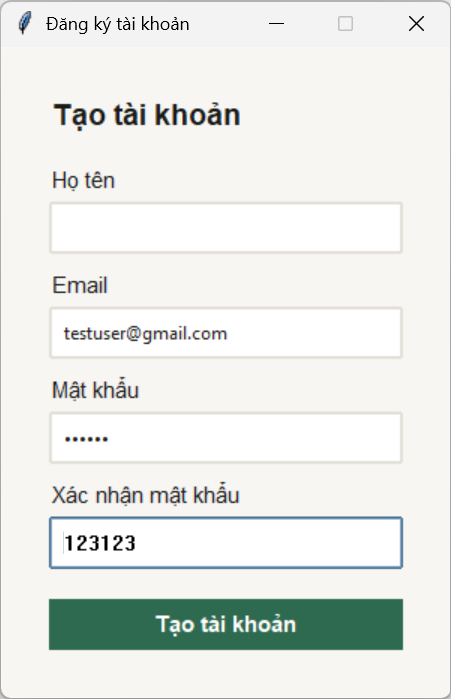
\includegraphics[width=0.9\linewidth]{IN_TC01.png}
        \par\vspace{0.1cm} 
        
        
\includegraphics[width=0.9\linewidth]{OUT_TC01.png}
        \par\vspace{0.2cm}
        
        \small\textbf{TC-001} 
        \vspace{0.3cm}
    \end{minipage}
    & 
    % --- Ô BÊN PHẢI ---
    \begin{minipage}{\linewidth}
        \centering
        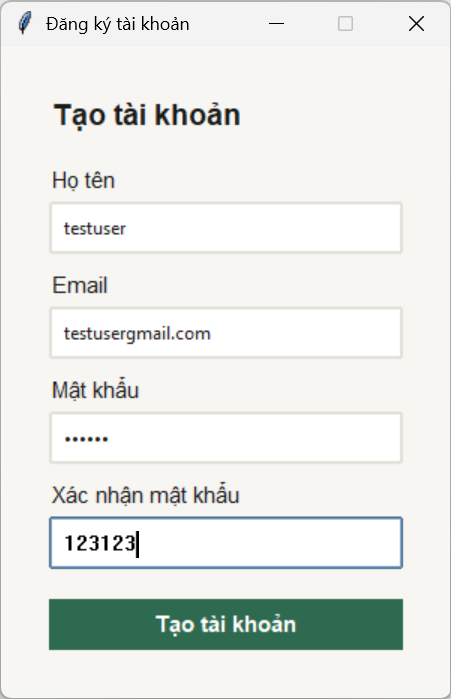
\includegraphics[width=0.9\linewidth]{IN_TC02.png}
        \par\vspace{0.1cm} 
        
        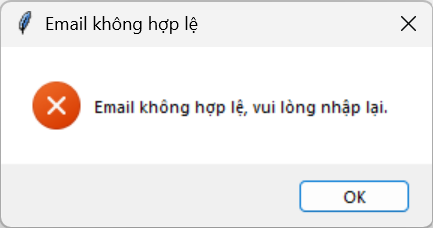
\includegraphics[width=0.9\linewidth]{OUT_TC02.png}
        \par\vspace{0.2cm}
        
        \small\textbf{TC-002} 
        \vspace{0.3cm}
    \end{minipage} \\
    
    \multicolumn{2}{c}{\vspace{0.5cm}} \\

    % ================= HÀNG 2 =================
    % --- Ô BÊN TRÁI ---
    \begin{minipage}{\linewidth}
        \centering
        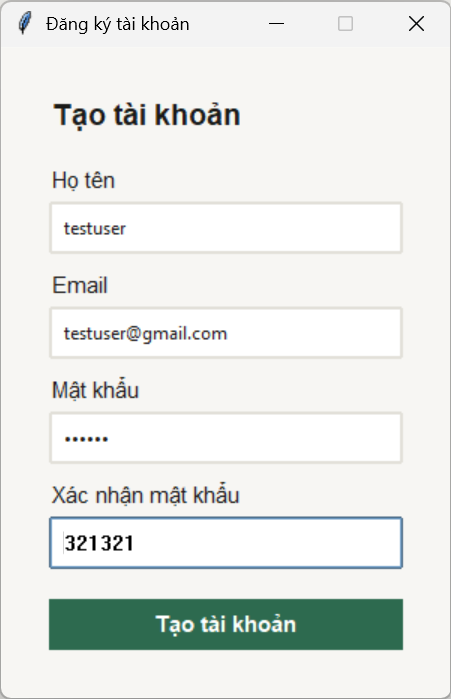
\includegraphics[width=0.9\linewidth]{IN_TC03.png}
        \par\vspace{0.1cm}
        
        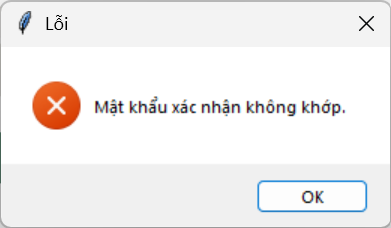
\includegraphics[width=0.9\linewidth]{OUT_TC03.png}
        \par\vspace{0.2cm}
        \small\textbf{TC-003}
        \vspace{0.3cm}
    \end{minipage} 
    & 
    % --- Ô BÊN PHẢI ---
    \begin{minipage}{\linewidth}
        \centering
        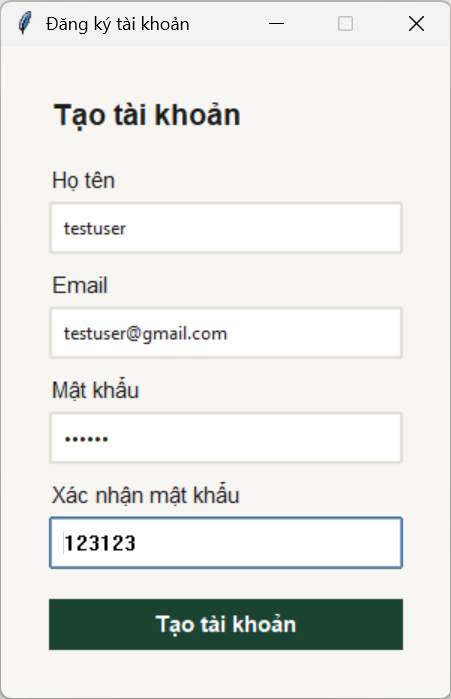
\includegraphics[width=0.9\linewidth]{IN_TC04.png}
        \par\vspace{0.1cm}
        
        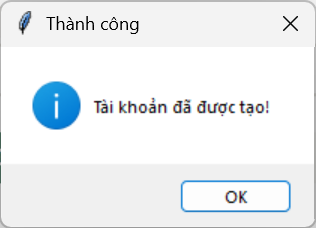
\includegraphics[width=0.9\linewidth]{OUT_TC04a.png}
        \par\vspace{0.2cm}
        \small\textbf{TC-004a} 
        \vspace{0.3cm}
    \end{minipage} \\

    % ================= HÀNG 3 (GỘP CỘT) =================
    \multicolumn{2}{c}{
        \begin{minipage}{\textwidth}
            \centering
            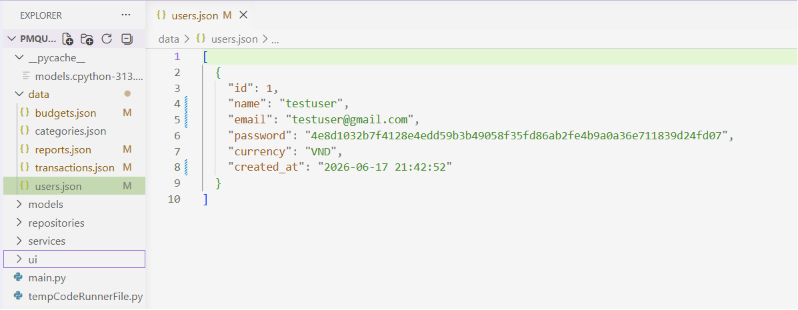
\includegraphics[width=\textwidth]{OUT_TC04b.png}
            \par\vspace{0.2cm}
            
            \small\textbf{TC-004b} 
            \vspace{0.3cm}
        \end{minipage}
    } \\

    % ================= HÀNG 4 (GỘP CỘT - 2 ẢNH XẾP DỌC) =================
    \multicolumn{2}{c}{
        \begin{minipage}{0.5\textwidth}
            \centering
            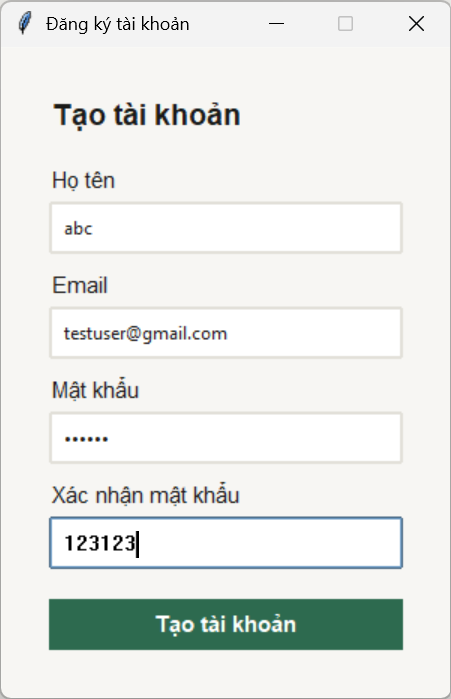
\includegraphics[width=0.85\textwidth]{IN_TC05.png}
            \par\vspace{0.2cm} 
            
            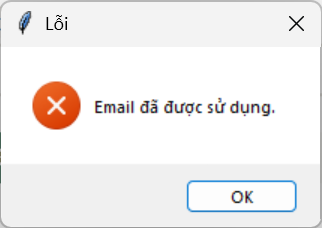
\includegraphics[width=0.85\textwidth]{OUT_TC05.png}
            \par\vspace{0.3cm} 
            
            \small\textbf{TC-005}
            \vspace{0.3cm}
        \end{minipage}
    } 
\end{xltabular}
\item \textbf{Đăng nhập tài khoản}
\renewcommand{\arraystretch}{1.5}
\begin{xltabular}{\textwidth}{|c|p{3.5cm}|X|p{3.5cm}|}
    \hline
    \centering\textbf{Mã} & \centering\textbf{Mô tả} & \centering\textbf{Input} & \centering\arraybackslash\textbf{Output mong muốn} \\
    \hline
    \endfirsthead
    \hline
    \centering\textbf{Mã} & \centering\textbf{Mô tả} & \centering\textbf{Input} & \centering\arraybackslash\textbf{Output mong muốn} \\
    \hline
    \endhead
    \endfoot
    \hline
    \caption{Bảng kiểm thử chức năng Đăng nhập }
    \label{tab:testcase_auth}
    \endlastfoot
    
    TC-006 & Email không tồn tại & \texttt{email="test@gmail.com", pw="123123"} & Hiện thông báo "Email hoặc mật khẩu sai" \\
    \hline
    TC-007 & Mật khẩu sai & \texttt{email="testusergmail.com", pw="321"} & Hiện thông báo "Email hoặc mật khẩu sai" \\
    \hline
    TC-008 & Đăng nhập thành công & \texttt{email="testuser@gmail.com", pw="123123"} & Tài khoản đăng nhập được, chuyển sang giao diện chính\\
\end{xltabular}

%Hình ảnh kết quả kiểm thử ĐĂNG NHẬP
\renewcommand{\arraystretch}{1.5}
\begin{xltabular}{\textwidth}{X X}
    % ================= HÀNG 1 =================
    \multicolumn{2}{c}{
        \begin{minipage}{\textwidth}
            \centering
            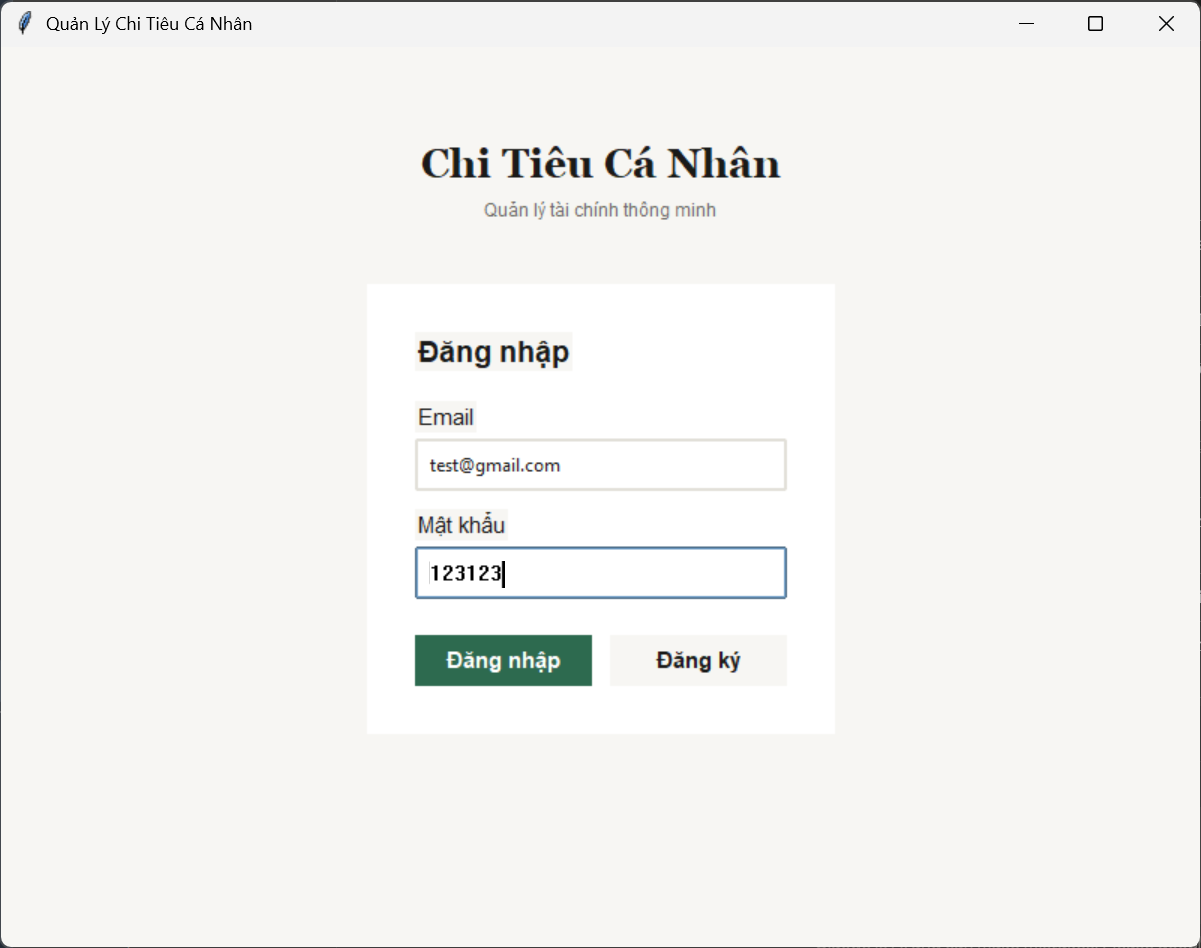
\includegraphics[width=0.85\textwidth]{IN_TC06.png}
            \par\vspace{0.2cm} 
            
            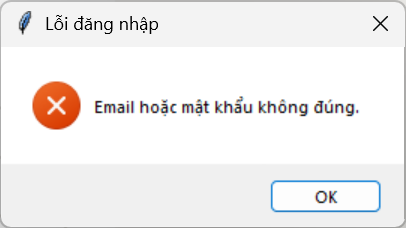
\includegraphics[width=0.6\textwidth]{OUT_TC06.png}
            \par\vspace{0.3cm} 
            
            \small\textbf{TC-006}
            \vspace{0.3cm}
        \end{minipage}
    }\\
        % ================= HÀNG 2 =================
    \multicolumn{2}{c}{
        \begin{minipage}{\textwidth}
            \centering
            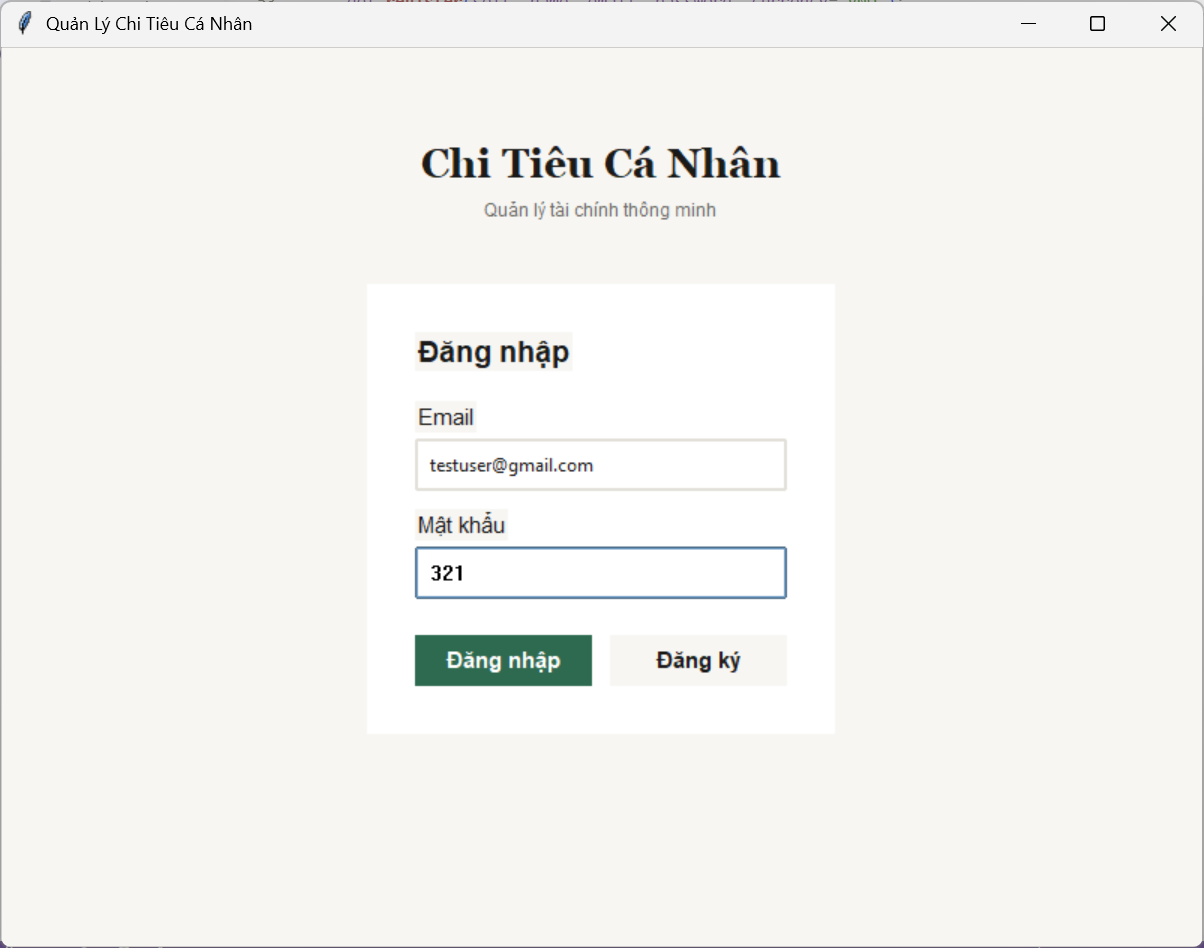
\includegraphics[width=0.85\textwidth]{IN_TC07.png}
            \par\vspace{0.2cm} 
            
            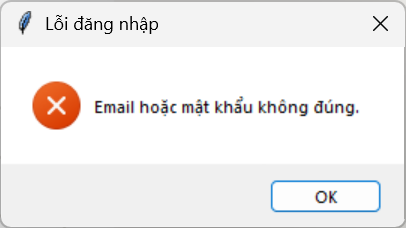
\includegraphics[width=0.6\textwidth]{OUT_TC07.png}
            \par\vspace{0.3cm} 
            
            \small\textbf{TC-007}
            \vspace{0.3cm}
        \end{minipage}
    }\\
    % ================= HÀNG 3 =================
    \multicolumn{2}{c}{
        \begin{minipage}{\textwidth}
            \centering
            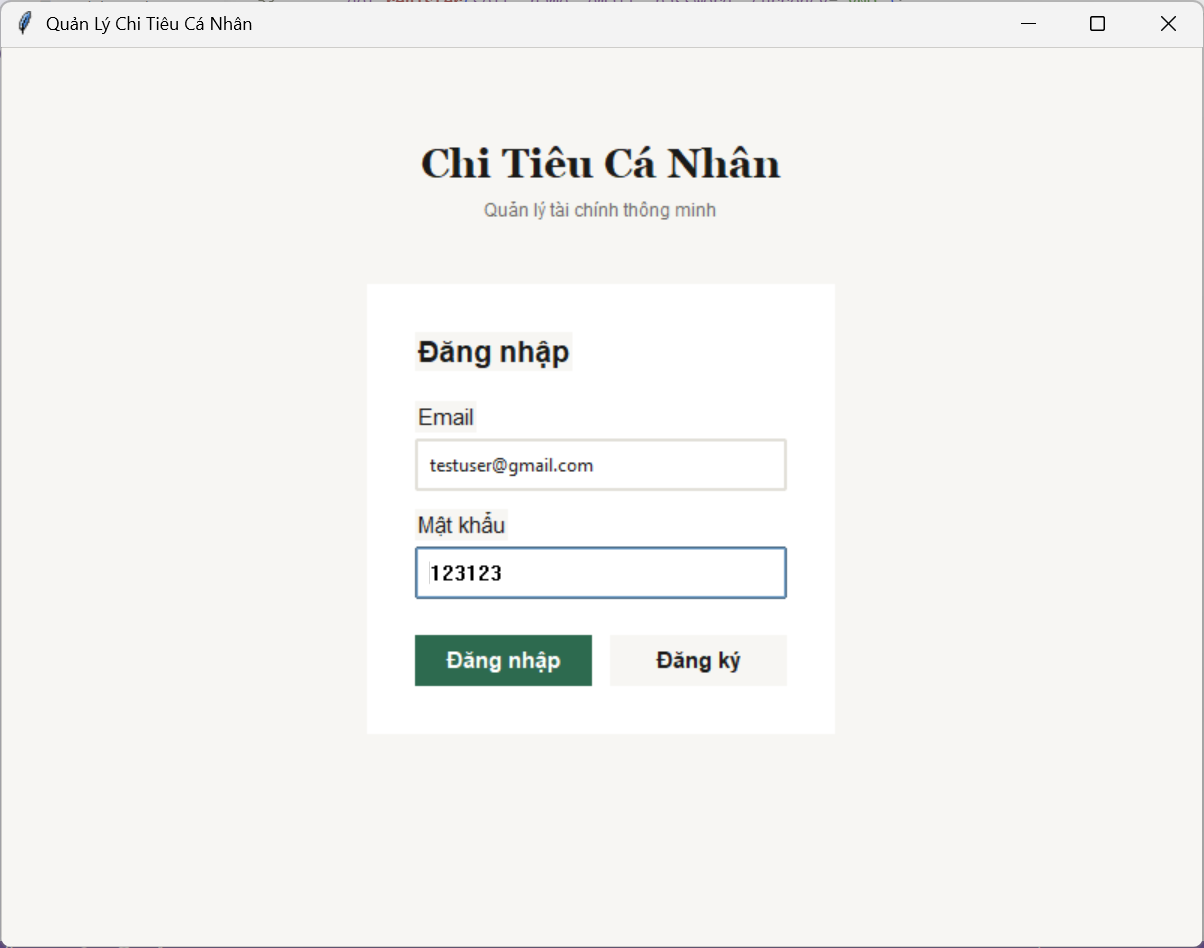
\includegraphics[width=0.85\textwidth]{IN_TC08.png}
            \par\vspace{0.2cm} 
            
            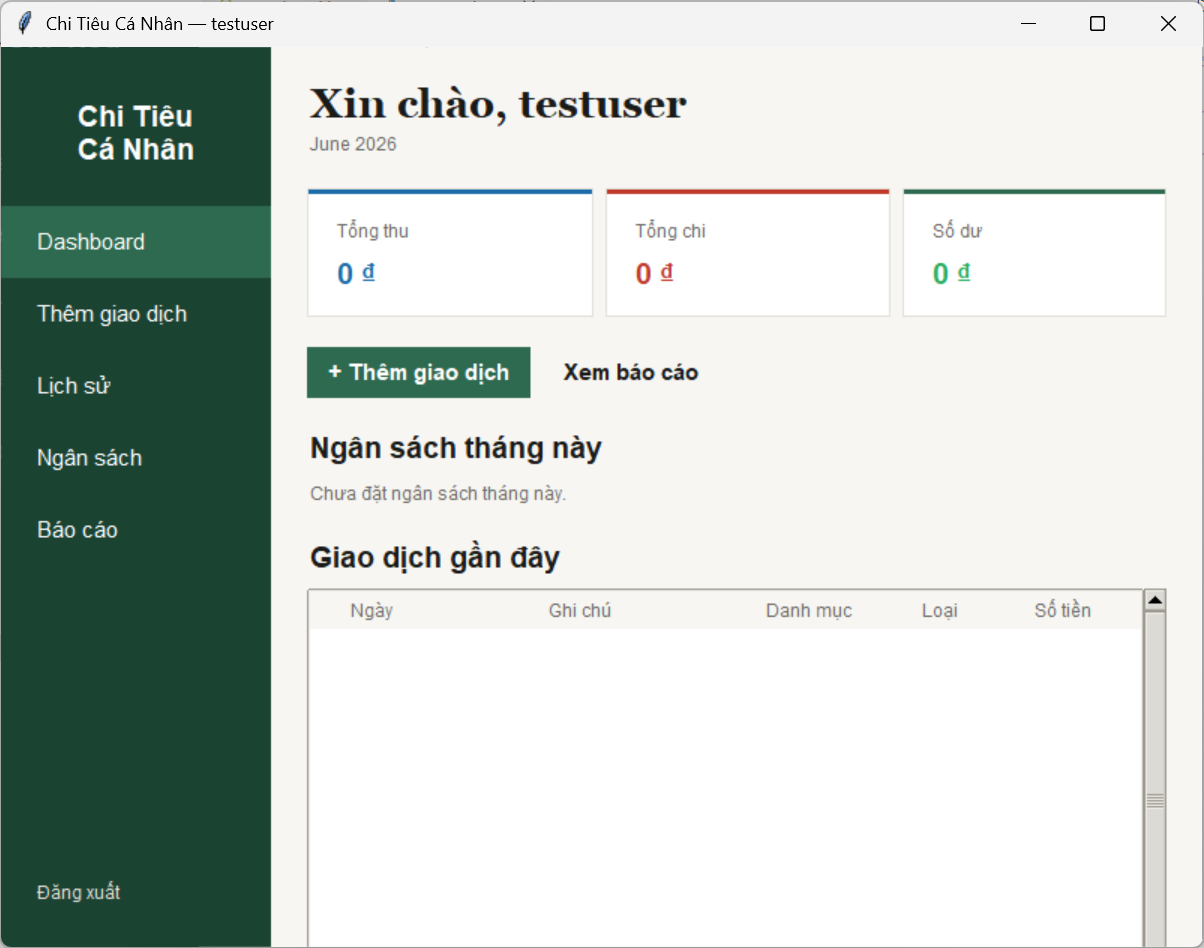
\includegraphics[width=0.85\textwidth]{OUT_TC08.png}
            \par\vspace{0.3cm} 
            
            \small\textbf{TC-008}
            \vspace{0.3cm}
        \end{minipage}
    } 
\end{xltabular}

\end{itemize}
\subsubsection{Chức năng 2: Thiết lập ngân sách}

Sau khi đã đăng nhập vào tài khoản, người dùng lựa chọn tab \texttt{Ngân sách} trên thanh công cụ bên trái giao diện để thực hiện các chức năng tạo lập/chỉnh sửa ngân sách cho từng loại danh mục.

\begin{xltabular}{\textwidth}{|c|p{3.5cm}|X|p{3.5cm}|}
    \hline
    \centering\textbf{Mã} & \centering\textbf{Mô tả} & \centering\textbf{Input} & \centering\arraybackslash\textbf{Output mong muốn} \\
    \hline
    \endfirsthead
    \hline
    \centering\textbf{Mã} & \centering\textbf{Mô tả} & \centering\textbf{Input} & \centering\arraybackslash\textbf{Output mong muốn} \\
    \hline
    \endhead
    \endfoot
    \hline
    \caption{Bảng kiểm thử chức năng Thiết lập ngân sách}
    \label{tab:testcase_auth}
    \endlastfoot
    TC-009& Số tiền sai định dạng & \texttt{month="2026-06", category= Ăn uống, limit\_amount= "abc"} & Hiện thông báo số tiền không hợp lệ \\
    \hline
    TC-010 & Thời gian sai định dạng & \texttt{month="2026-16", category= Ăn uống, limit\_amount= "123000"} & Hiện thông báo lỗi về tháng \\
    \hline
    TC-011 & Thiết lập ngân sách thành công & \texttt{month="2026-06", category= Ăn uống, limit\_amount= "123000"} & Hiện thông báo thiết lập thành công \\
    \hline
    TC-012 & Chỉnh sửa ngân sách cho một danh mục đã có ngân sách trước đó & \texttt{month="2026-06", category= Ăn uống, limit\_amount= "100000"} & Hiện thông báo thiết lập thành công \\
    \hline
\end{xltabular}

% Hình ảnh kết quả kiểm thử NGÂN SÁCH
\begin{center}
    % ================= TC-009 =================
    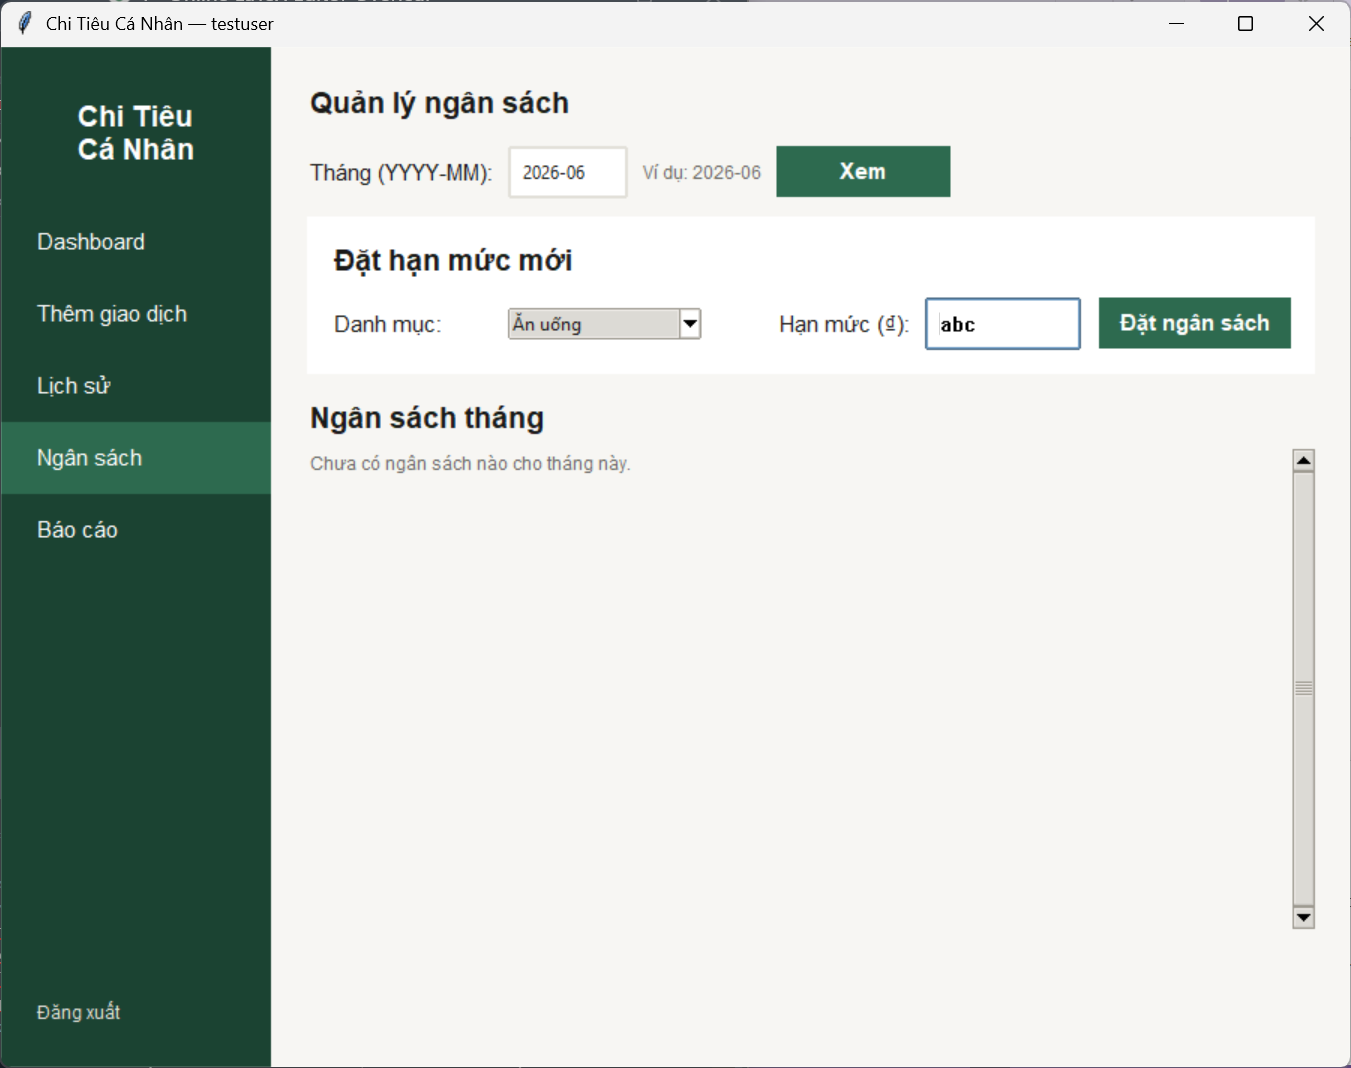
\includegraphics[width=0.85\textwidth]{IN_TC09.png}
    \par\vspace{0.2cm} 
    
    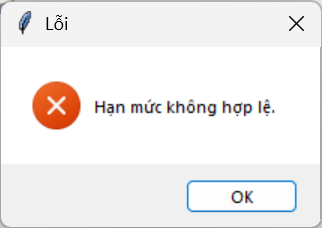
\includegraphics[width=0.6\textwidth]{OUT_TC09.png}
    \par\vspace{0.3cm} 
    
    \small\textbf{TC-009}
    \par\vspace{0.8cm} % Khoảng cách giữa các TC

    % ================= TC-010 =================
    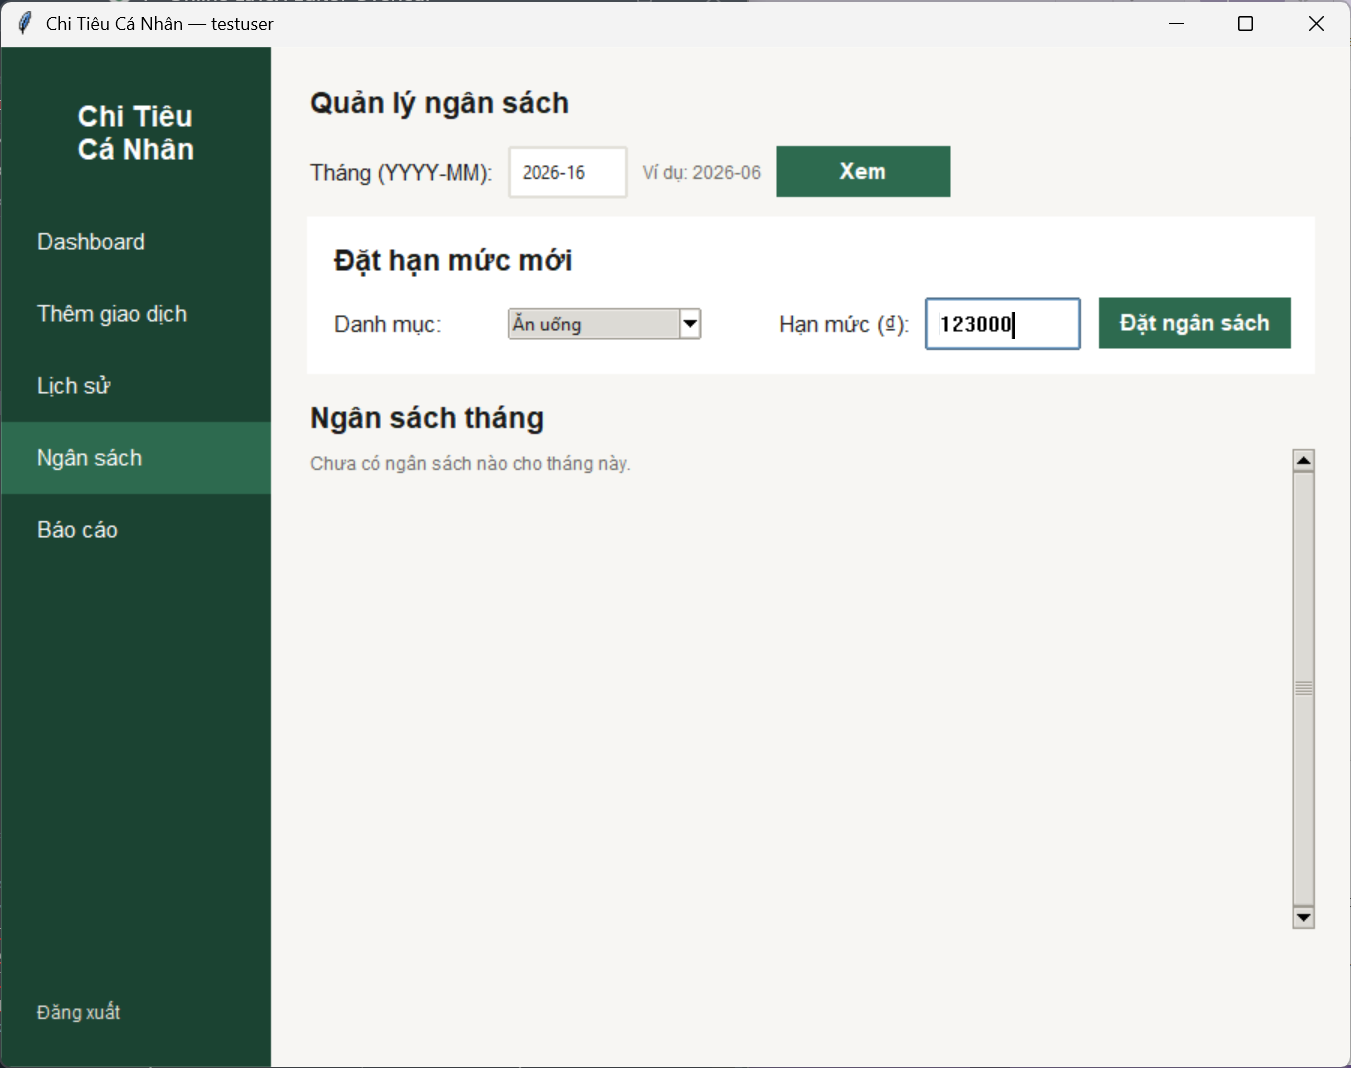
\includegraphics[width=0.85\textwidth]{IN_TC10.png}
    \par\vspace{0.2cm} 
    
    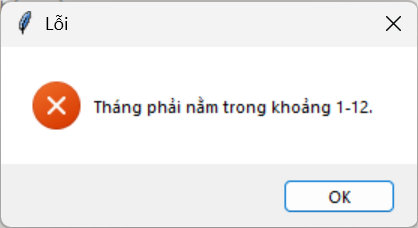
\includegraphics[width=0.6\textwidth]{OUT_TC10.png}
    \par\vspace{0.3cm} 
    
    \small\textbf{TC-010}
    \par\vspace{0.8cm}

    % ================= TC-011 =================
    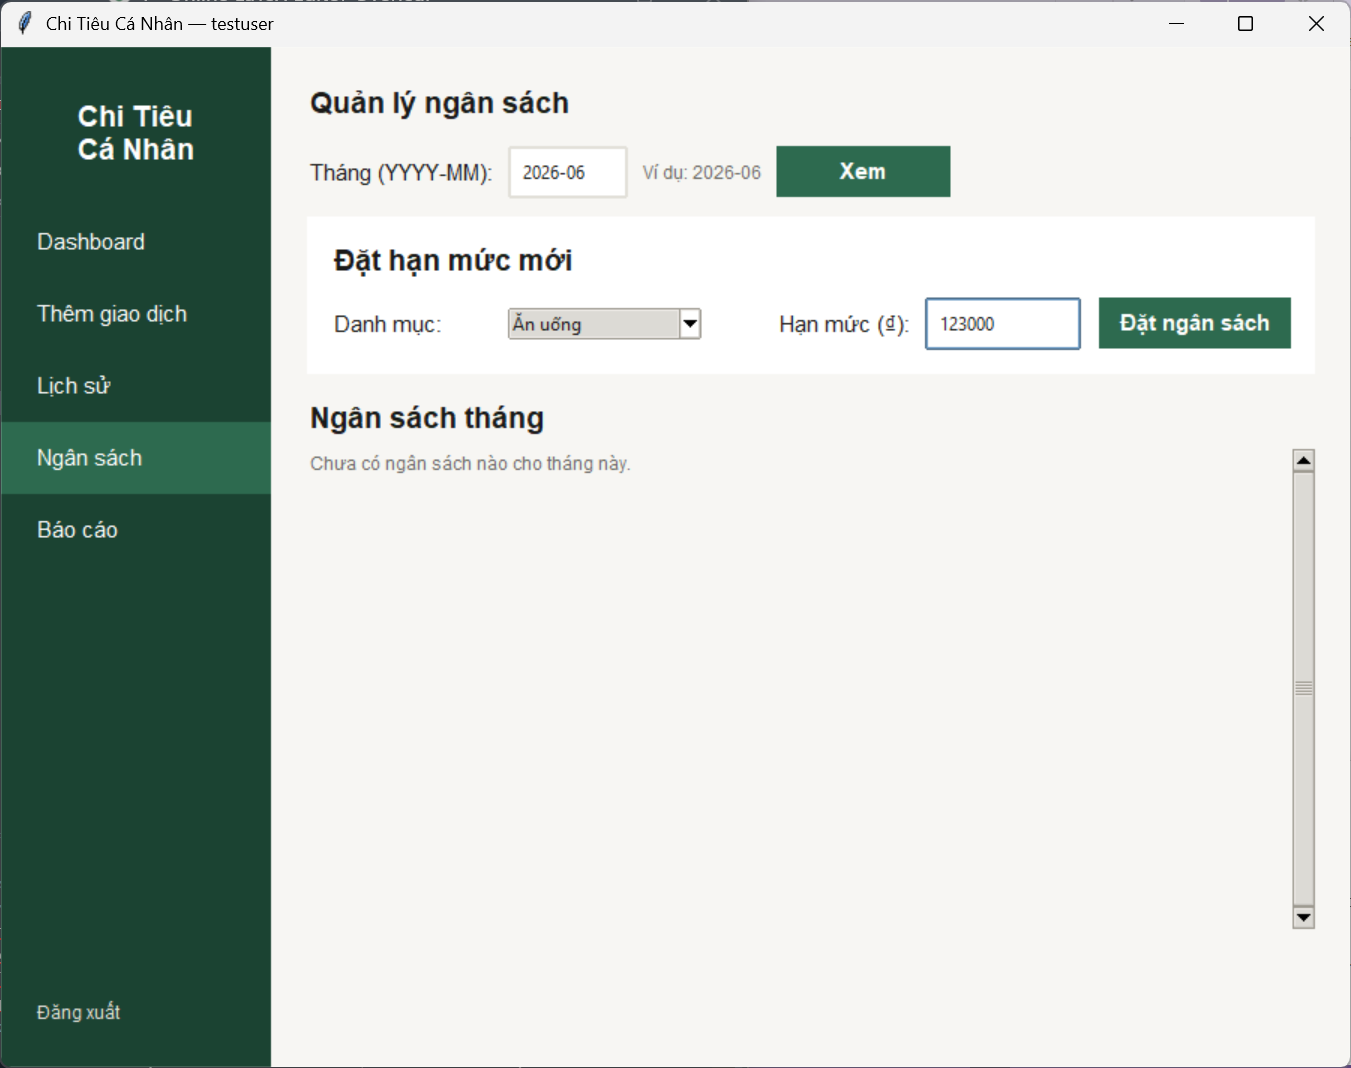
\includegraphics[width=0.85\textwidth]{IN_TC11.png}
    \par\vspace{0.2cm} 
    
    
\includegraphics[width=0.5\textwidth]{OUT_TC11a.png}
    \par\vspace{0.3cm} 

    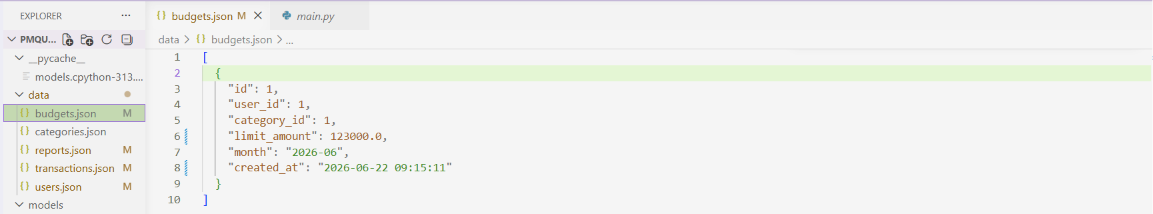
\includegraphics[width=\textwidth]{OUT_TC11b.png}
    \par\vspace{0.3cm} 

    \small\textbf{TC-011}
    \par\vspace{0.8cm}

    % ================= TC-012 =================
    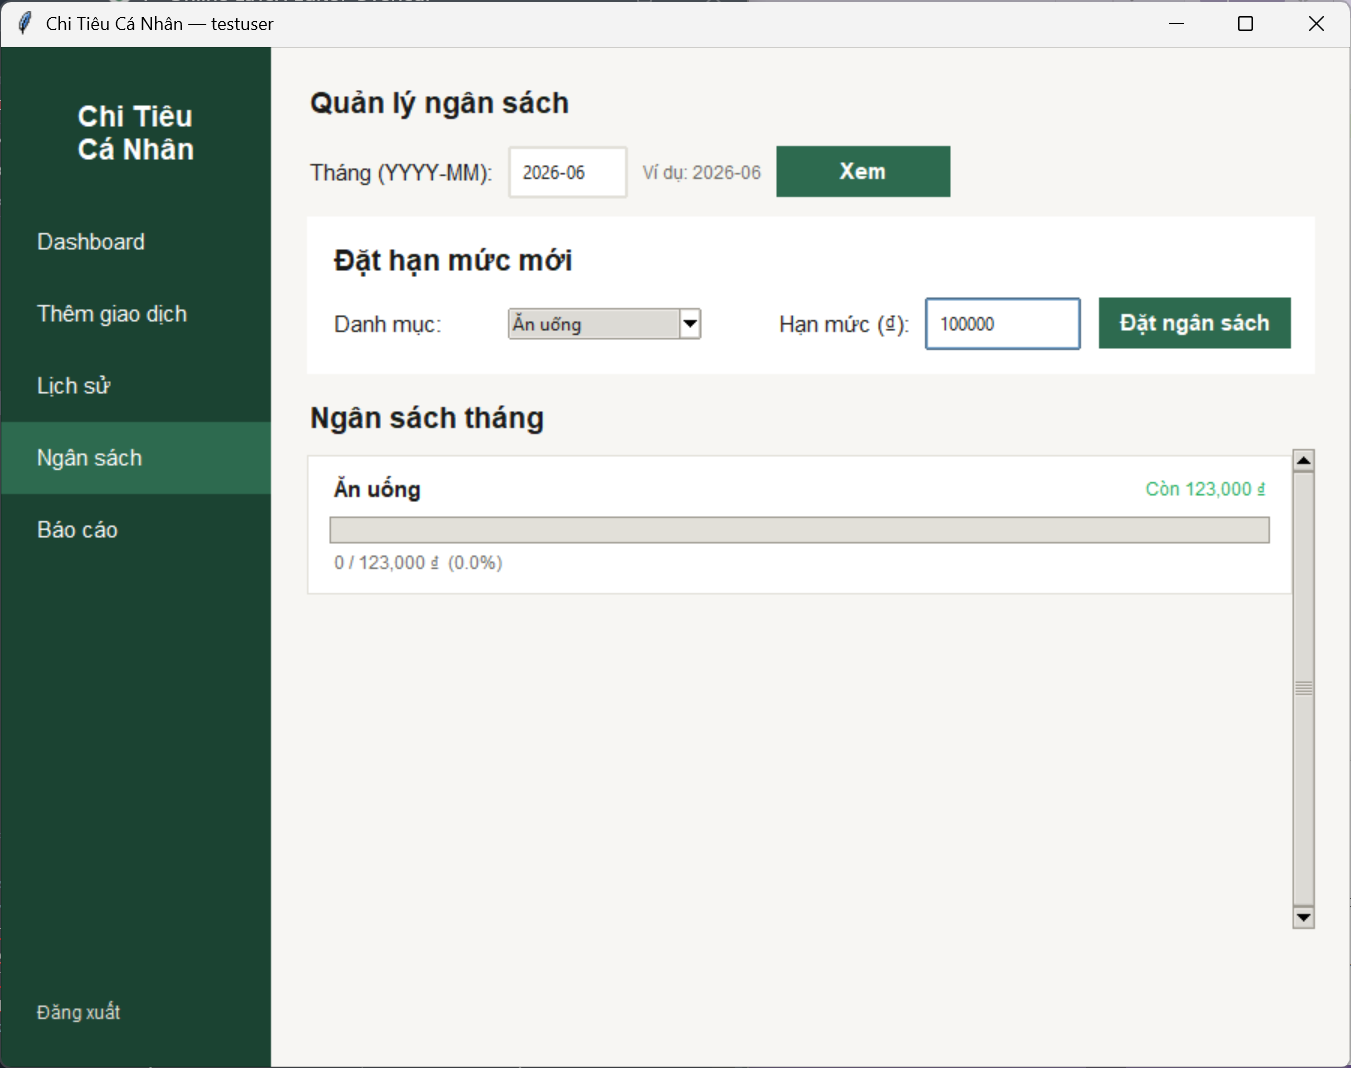
\includegraphics[width=0.85\textwidth]{IN_TC12.png}
    \par\vspace{0.2cm} 
    
    
\includegraphics[width=0.5\textwidth]{OUT_TC12a.png}
    \par\vspace{0.3cm} 

    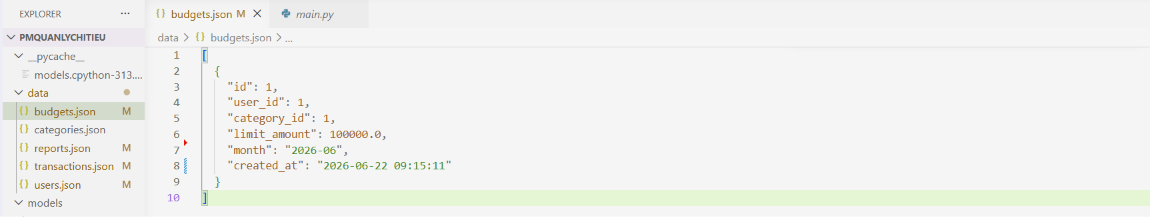
\includegraphics[width=\textwidth]{OUT_TC12b.png}
    \par\vspace{0.3cm} 

    \small\textbf{TC-012}
    \vspace{0.3cm}
\end{center}\subsubsection{Chức năng 3: Ghi chép giao dịch}
Sau khi đăng nhập vào tài khoản, tại tab Dashboard người dùng có thể lựa chọn nút chức năng thêm giao dịch hoặc lựa chọn tab Thêm giao dịch để thực hiện chức năng này. Với ngân sách của danh mục Ăn uống đã được thiết lập ở trên, thực hiện các test case như bên dưới.
\begin{itemize}
    \item Thêm giao dịch
    \begin{xltabular}{\textwidth}{|c|p{3.5cm}|X|p{3.5cm}|}
    \hline
    \centering\textbf{Mã} & \centering\textbf{Mô tả} & \centering\textbf{Input} & \centering\arraybackslash\textbf{Output mong muốn} \\
    \hline
    \endfirsthead
    \hline
    \centering\textbf{Mã} & \centering\textbf{Mô tả} & \centering\textbf{Input} & \centering\arraybackslash\textbf{Output mong muốn} \\
    \hline
    \endhead
    \endfoot
    \hline
    \caption{Bảng kiểm thử chức năng Thêm giao dịch}
    \label{tab:testcase_auth}
    \endlastfoot
    TC-013& Số tiền sai định dạng & \texttt{type= Chi tiêu, category= Ăn uống, amount= "abc", date="2026-06-22", note=""} & Hiện thông báo số tiền không hợp lệ \\
    \hline
    TC-014 & Thời gian sai định dạng & \texttt{type= Chi tiêu, category= Ăn uống, amount= "120000", date="2026-06-35", note=""} & Hiện thông báo lỗi về thời gian \\
    \hline
    TC-015 & Nhập vào một chi tiêu vượt ngân sách & \texttt{type= Chi tiêu, category= Ăn uống, amount= "120000", date="2026-06-22", note=""} & Hiện cảnh báo vượt ngân sách và thông báo thiết lập thành công \\
    \hline
    TC-016& Nhâp vào một khoản thu nhập & \texttt{type= Thu nhập, category= Tiền lương, amount= "5000000", date="2026-06-22", note=""} & Hiện thông nhập vào thành công \\
    \hline
\end{xltabular}

%Hình ảnh kết quả kiểm thử Thêm giao dịch
\renewcommand{\arraystretch}{1.5}
\begin{xltabular}{\textwidth}{X X}
    % ================= HÀNG 1 =================
    \multicolumn{2}{c}{
        \begin{minipage}{\textwidth}
            \centering
            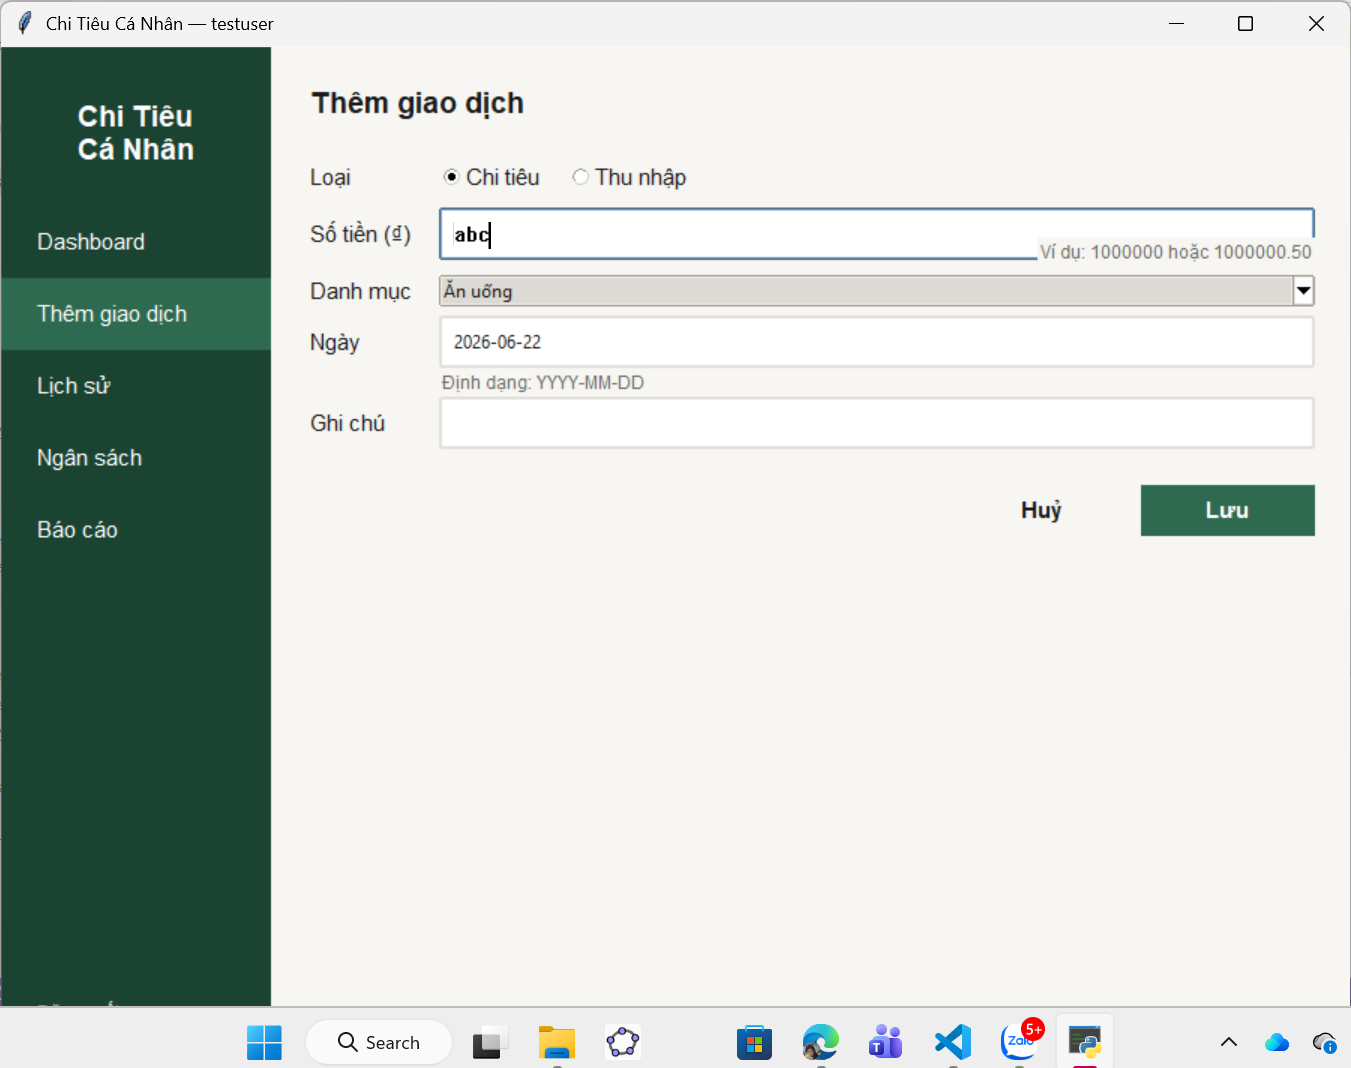
\includegraphics[width=0.85\textwidth]{IN_TC13.png}
            \par\vspace{0.2cm} 
            
            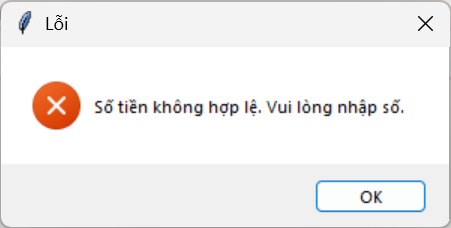
\includegraphics[width=0.6\textwidth]{OUT_TC13.png}
            \par\vspace{0.3cm} 
            
            \small\textbf{TC-013}
            \vspace{0.3cm}
        \end{minipage}
    }\\
        % ================= HÀNG 2 =================
    \multicolumn{2}{c}{
        \begin{minipage}{\textwidth}
            \centering
            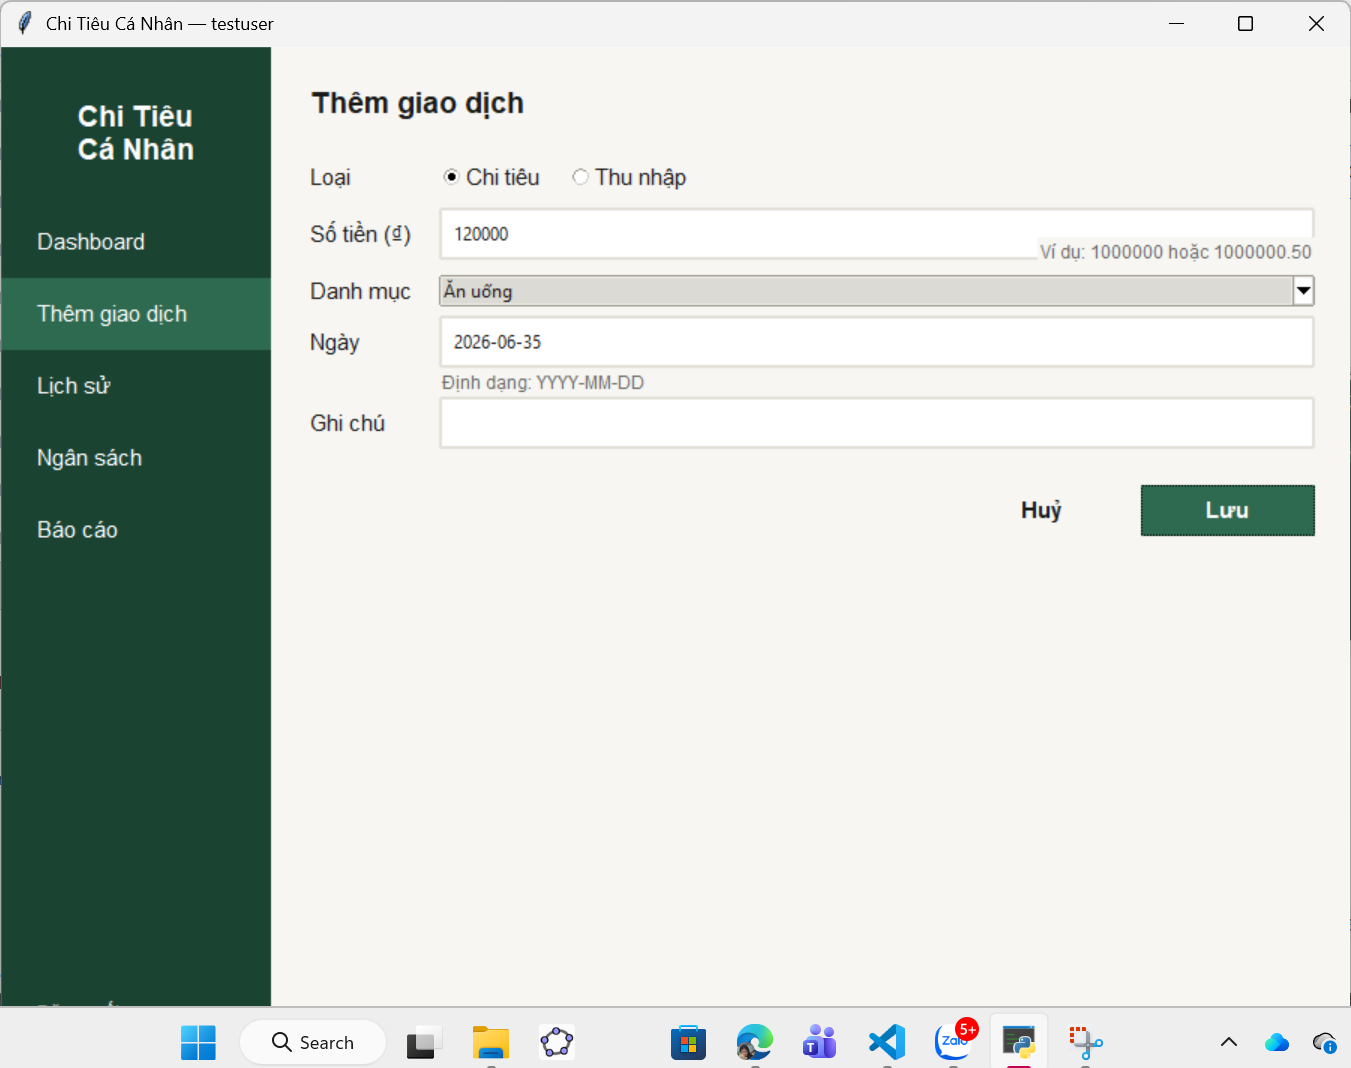
\includegraphics[width=0.85\textwidth]{IN_TC14.png}
            \par\vspace{0.2cm} 
            
            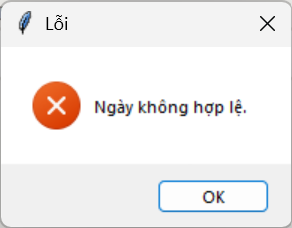
\includegraphics[width=0.5\textwidth]{OUT_TC14.png}
            \par\vspace{0.3cm} 
            
            \small\textbf{TC-014}
            \vspace{0.3cm}
        \end{minipage}
    }\\
    % ================= HÀNG 3 =================
    \multicolumn{2}{c}{
        \begin{minipage}{\textwidth}
            \centering
            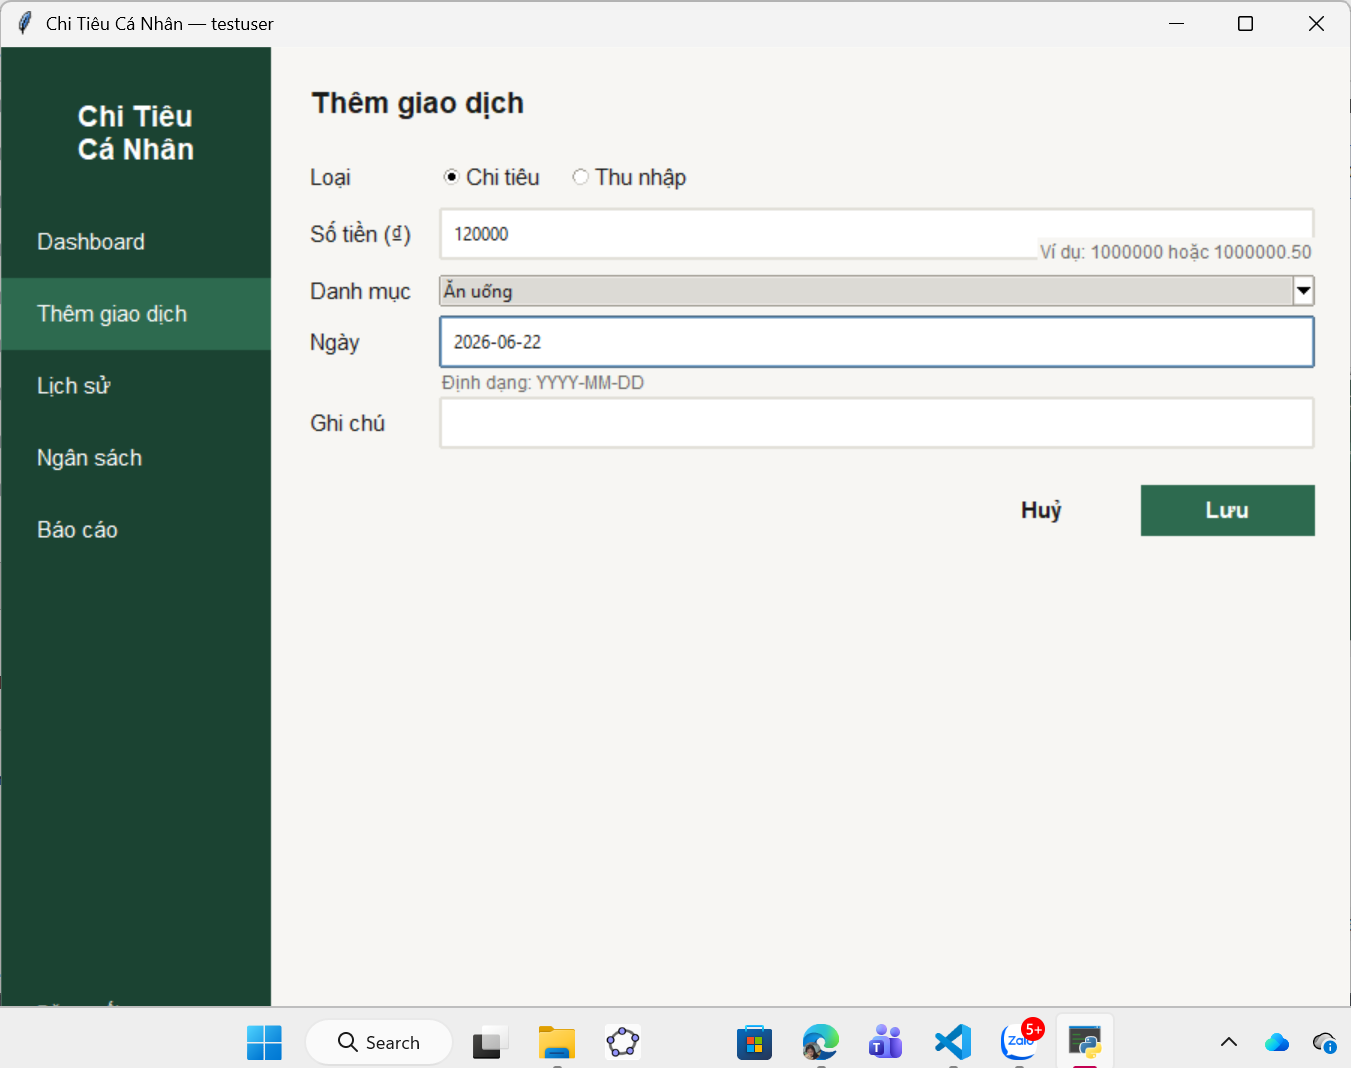
\includegraphics[width=0.85\textwidth]{IN_TC15.png}
            \par\vspace{0.2cm} 
            
            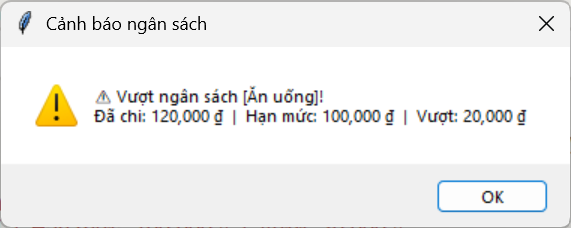
\includegraphics[width=0.6\textwidth]{OUT_TC15a.png}
            \par\vspace{0.3cm} 

            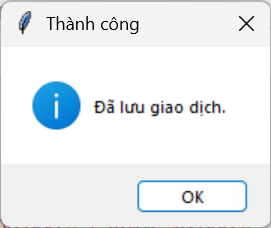
\includegraphics[width=0.3\textwidth]{OUT_TC15b.png}
            \par\vspace{0.3cm} 

            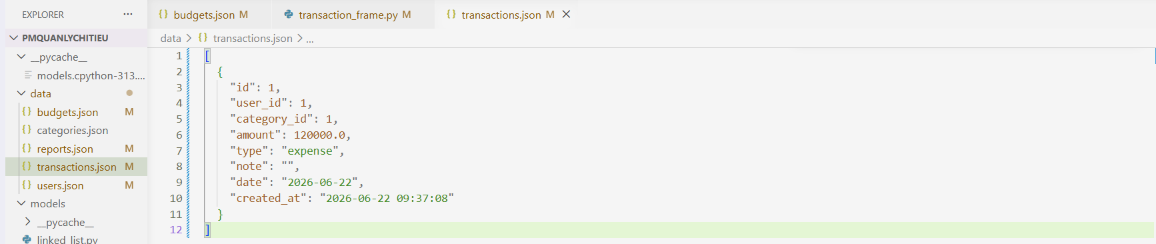
\includegraphics[width=\textwidth]{OUT_TC15c.png}
            \par\vspace{0.3cm} 

            \small\textbf{TC-015}
            \vspace{0.3cm}
        \end{minipage}
    }\\
        % ================= HÀNG 4 =================
    \multicolumn{2}{c}{
        \begin{minipage}{\textwidth}
            \centering
            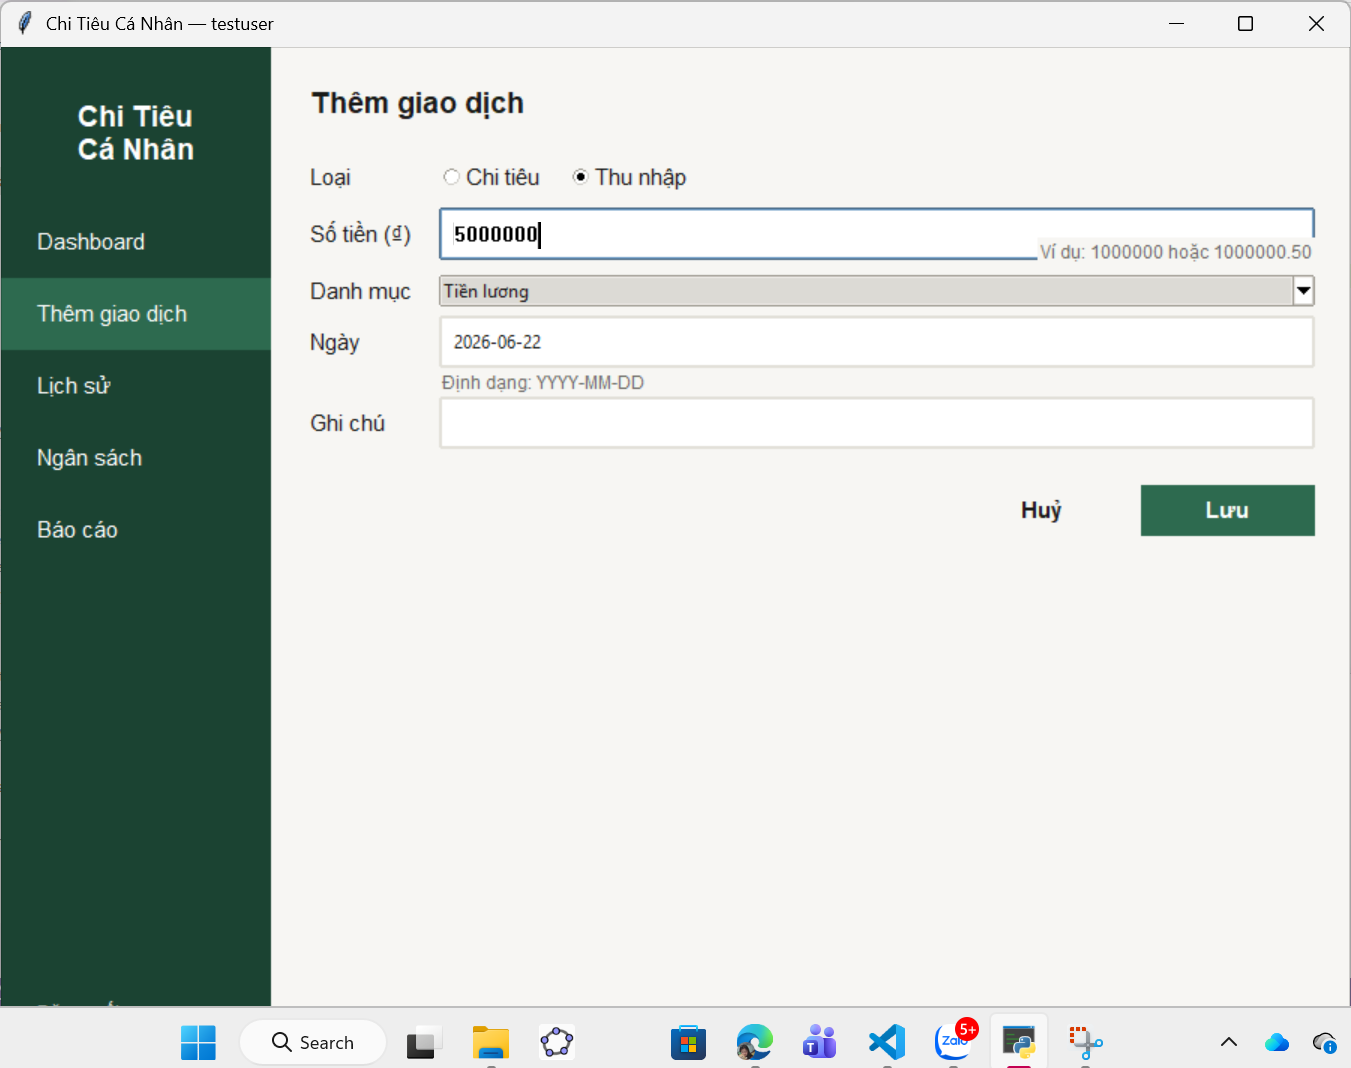
\includegraphics[width=0.85\textwidth]{IN_TC16.png}
            \par\vspace{0.2cm} 
            
            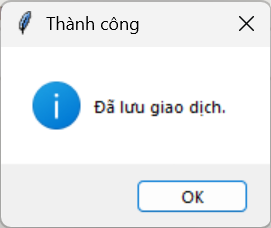
\includegraphics[width=0.45\textwidth]{OUT_TC16a.png}
            \par\vspace{0.3cm} 

            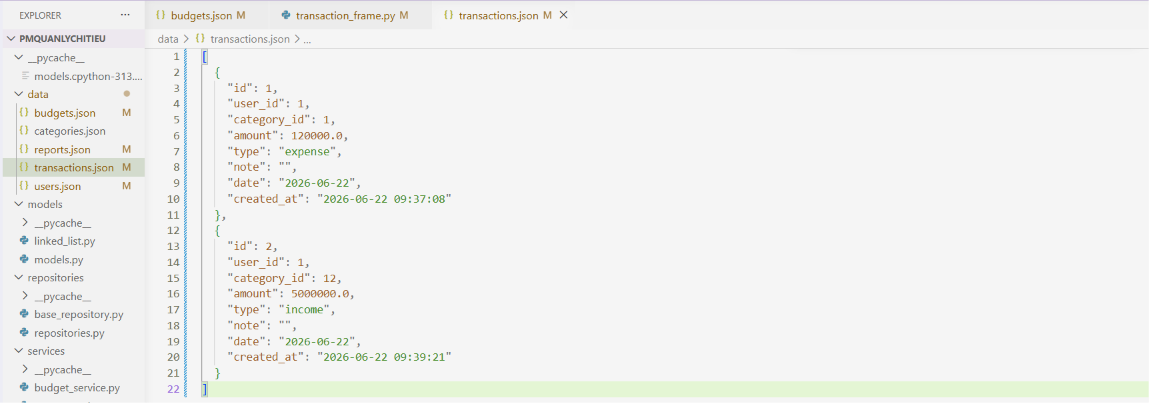
\includegraphics[width=\textwidth]{OUT_TC16b.png}
            \par\vspace{0.3cm} 

            \small\textbf{TC-016}
            \vspace{0.3cm}
        \end{minipage}
    } 
\end{xltabular}
    \item Xóa giao dịch
Để thực hiện xóa một giao dịch, người dùng lựa chọn tab \texttt{Lịch sử}, click vào giao dịch muốn xóa và chọn vào nút xóa ở góc phải giao diện.
\begin{xltabular}{\textwidth}{|c|p{3.5cm}|X|p{3.5cm}|}
\hline
\centering\textbf{Mã} & \centering\textbf{Mô tả} & \centering\textbf{Input} & \centering\arraybackslash\textbf{Output mong muốn} \\
\hline
TC-017& Xóa một giao dịch & Chọn một giao dịch trong tab lịch sử & Giao dịch được xóa khỏi hệ thống \\
\hline
\end{xltabular}

% Hình ảnh kết quả kiểm thử Xóa giao dịch
\begin{center}
    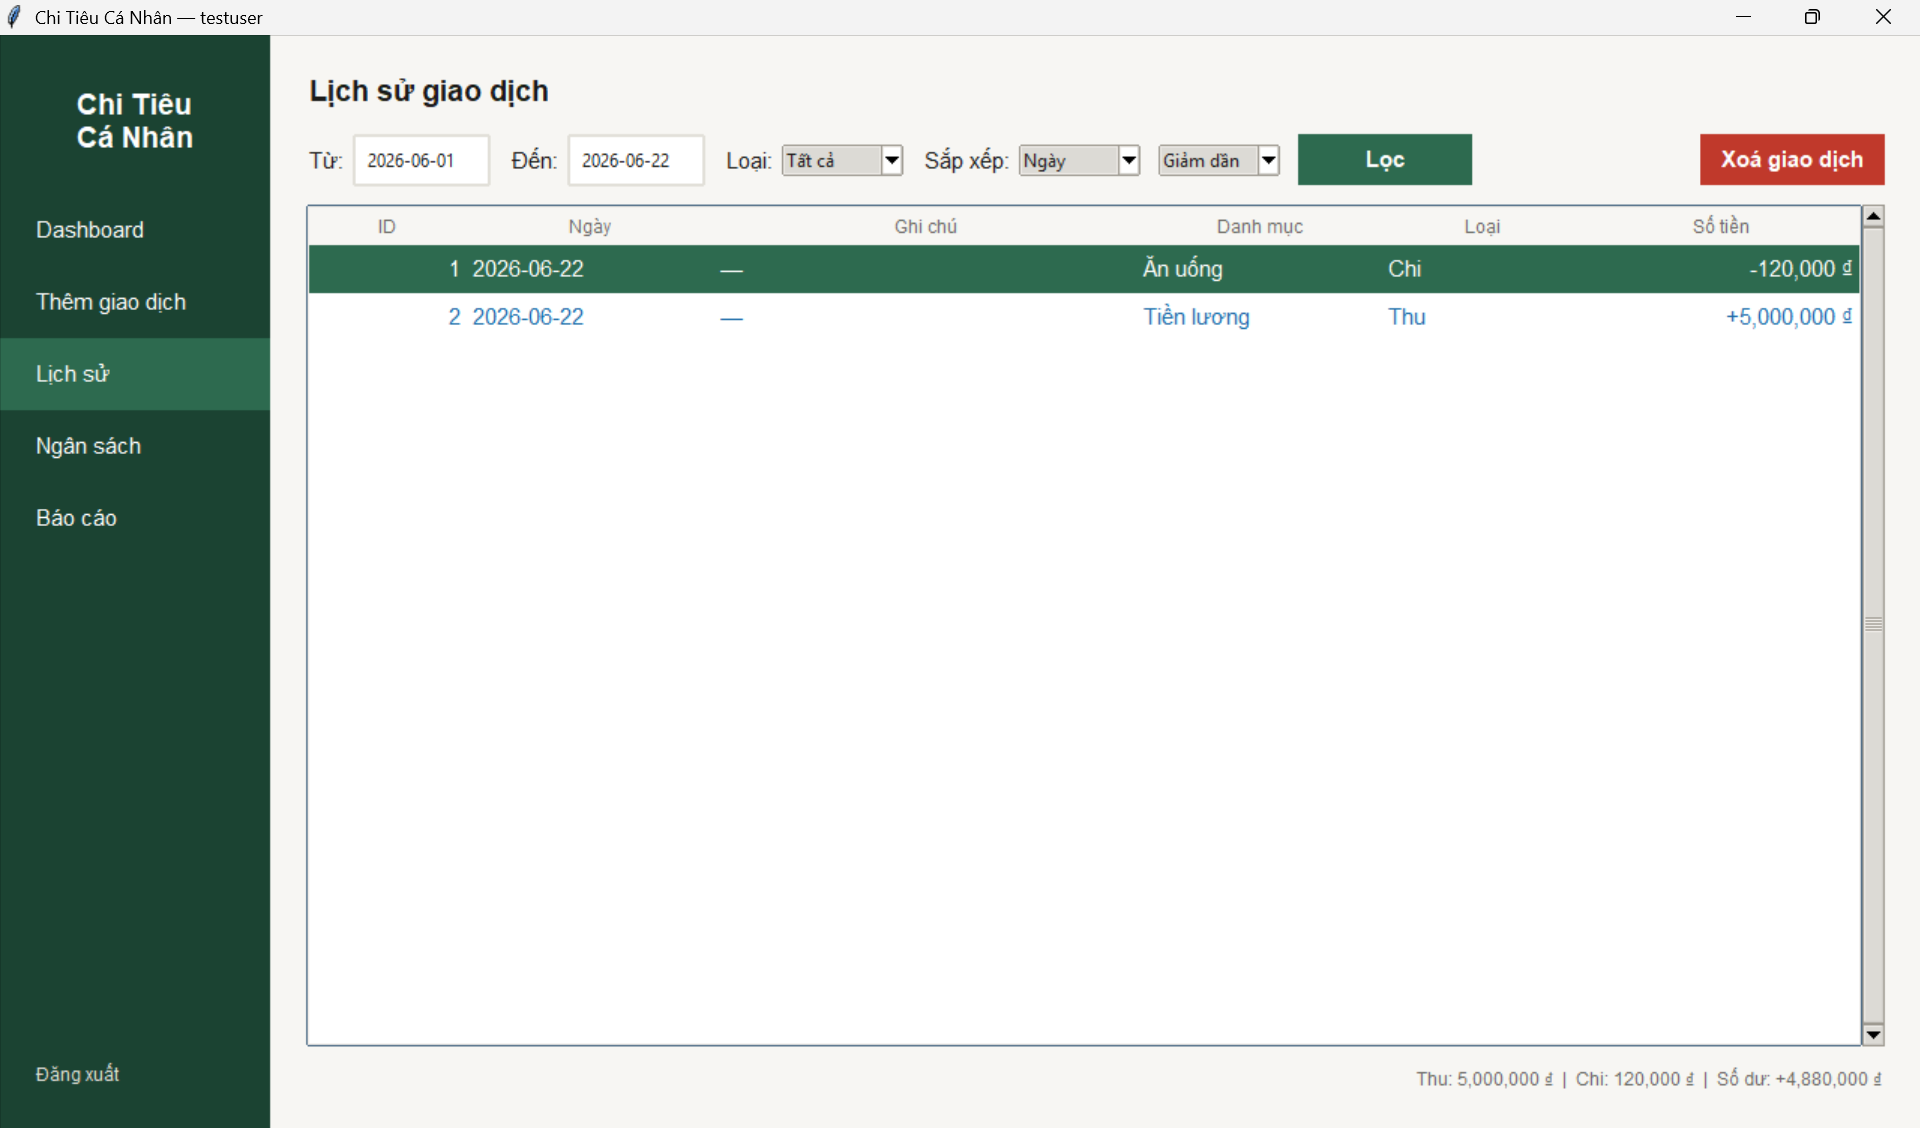
\includegraphics[width=0.85\textwidth]{IN_TC17a.png}
    \par\vspace{0.2cm} 

    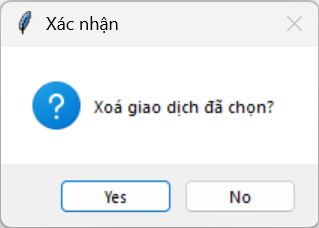
\includegraphics[width=0.4\textwidth]{IN_TC17b.png}
    \par\vspace{0.2cm} 

    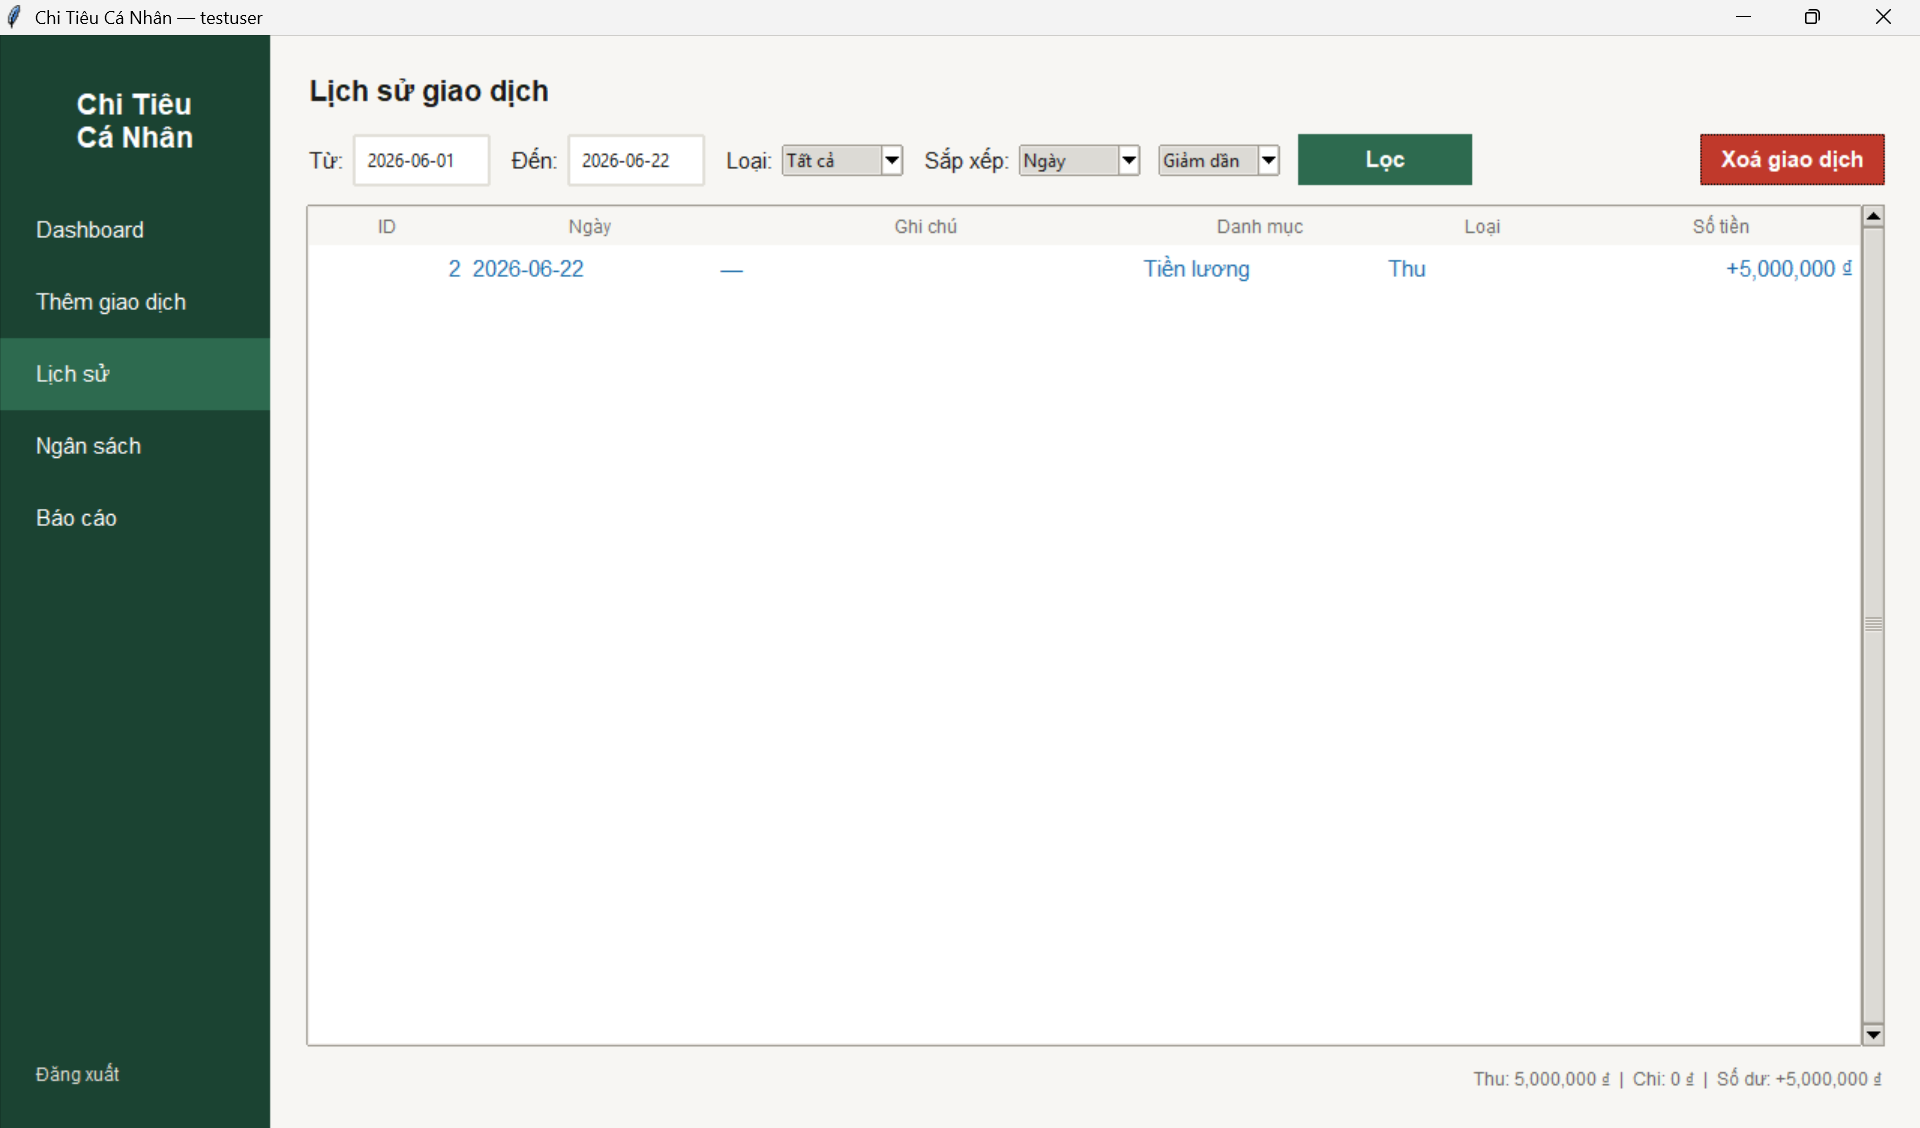
\includegraphics[width=0.85\textwidth]{OUT_TC17a.png}
    \par\vspace{0.3cm} 

    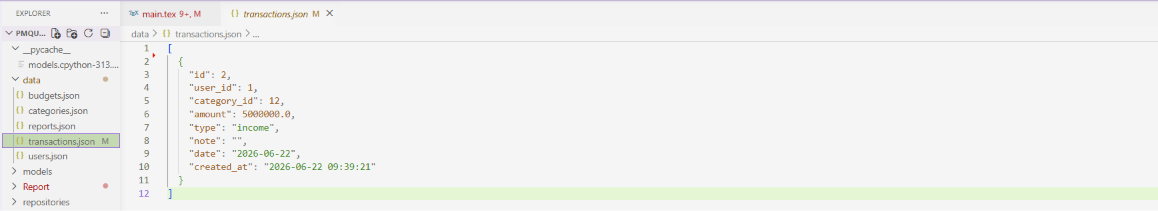
\includegraphics[width=\textwidth]{OUT_TC17b.png}
    \par\vspace{0.3cm} 

    \small\textbf{TC-017}
    \vspace{0.3cm}
\end{center}
\end{itemize}
\subsubsection{Chức năng 4: Báo cáo chi tiêu}
Sau khi đã nhập các giao dịch cũng như ngân sách các danh mục vào hệ thống, người dùng sẽ có thể xem báo cáo thu chi tại tab \texttt{Báo cáo}. Khi test chức năng này, chúng em sử dụng file data test để thiết lập một số lượng giao dịch và ngân sách đủ lớn để có dữ liệu sinh báo cáo.
    \begin{xltabular}{\textwidth}{|c|p{3.5cm}|X|p{3.5cm}|}
    \hline
    \centering\textbf{Mã} & \centering\textbf{Mô tả} & \centering\textbf{Input} & \centering\arraybackslash\textbf{Output mong muốn} \\
    \hline
    \endfirsthead
    \hline
    \centering\textbf{Mã} & \centering\textbf{Mô tả} & \centering\textbf{Input} & \centering\arraybackslash\textbf{Output mong muốn} \\
    \hline
    \endhead
    \endfoot
    \hline
    \caption{Bảng kiểm thử chức năng Báo cáo chi tiêu}
    \label{tab:testcase_auth}
    \endlastfoot
    TC-018& Báo cáo theo tháng & \texttt{period\_type= month} & Hiện báo cáo cho tháng hiện tại \\
    \hline
    TC-019 & Báo cáo theo quý & \texttt{period\_type= quarter} & Hiện báo cáo cho quý hiện tại \\
    \hline
    TC-020& Báo cáo theo năm & \texttt{period\_type= year} & Hiện báo cáo cho năm hiện tại \\
    \hline
    TC-021 & Báo cáo chi tiêu một khoảng thời gian tùy chọn & \texttt{start\_date: "2026-06-01", end\_date: "2026-06-15"} & Báo cáo chi tiêu cho khoảng thời gian đó \\
    \hline
    \end{xltabular}
% Hình ảnh kết quả kiểm thử Báo cáo chi tiêu
\begin{center}
    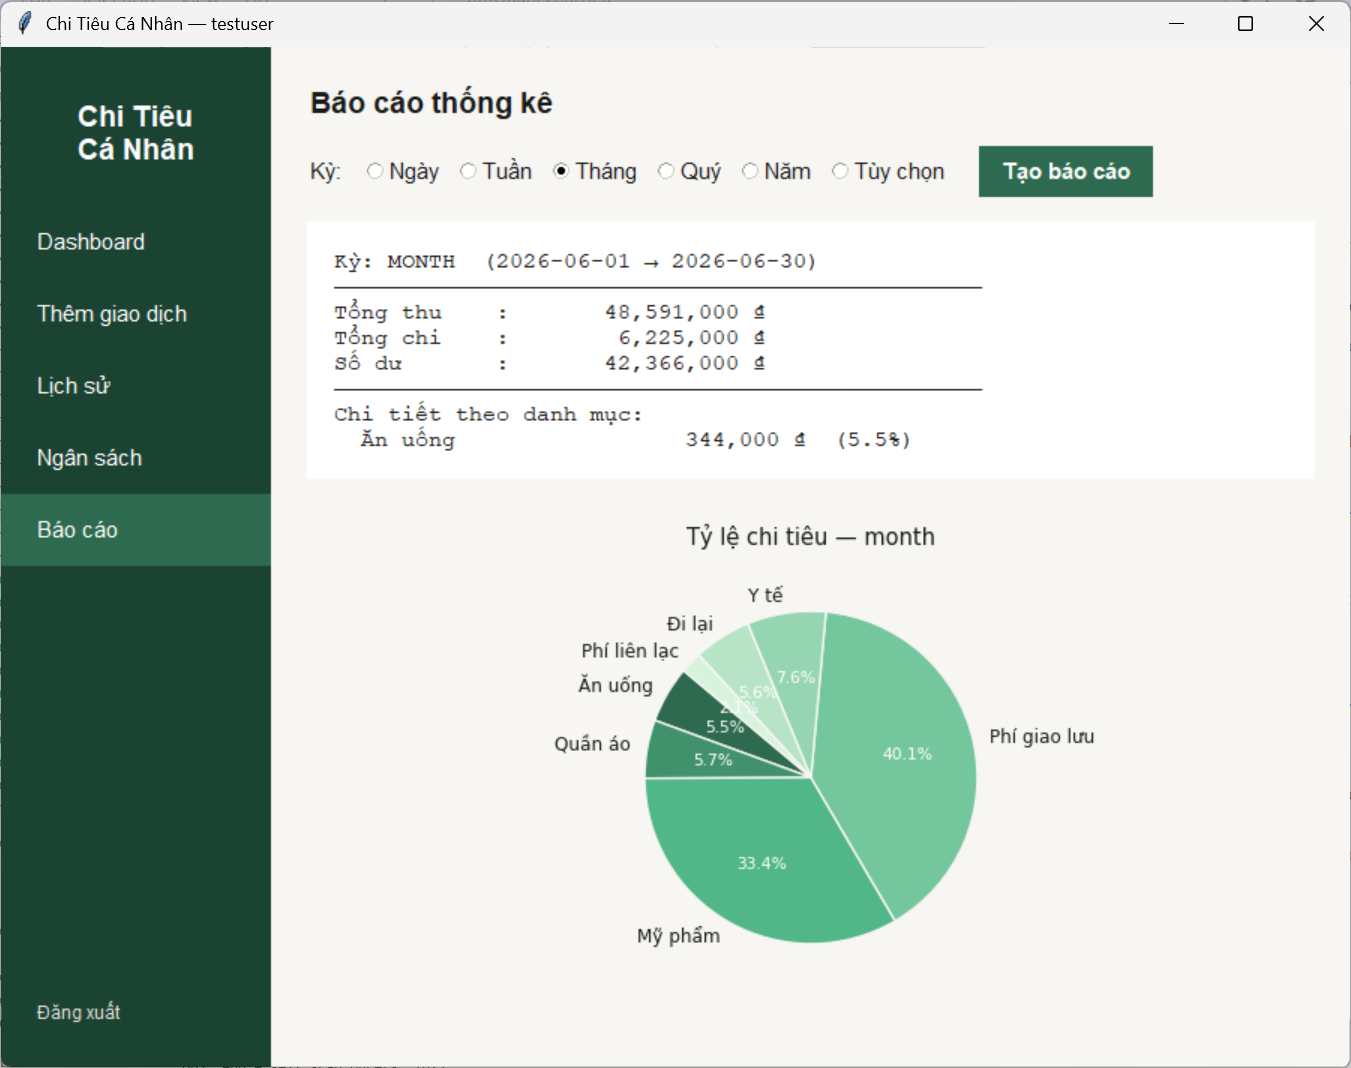
\includegraphics[width=0.85\textwidth]{OUT_TC18.png}
    \par\vspace{0.2cm} 
    \small\textbf{TC-018}

    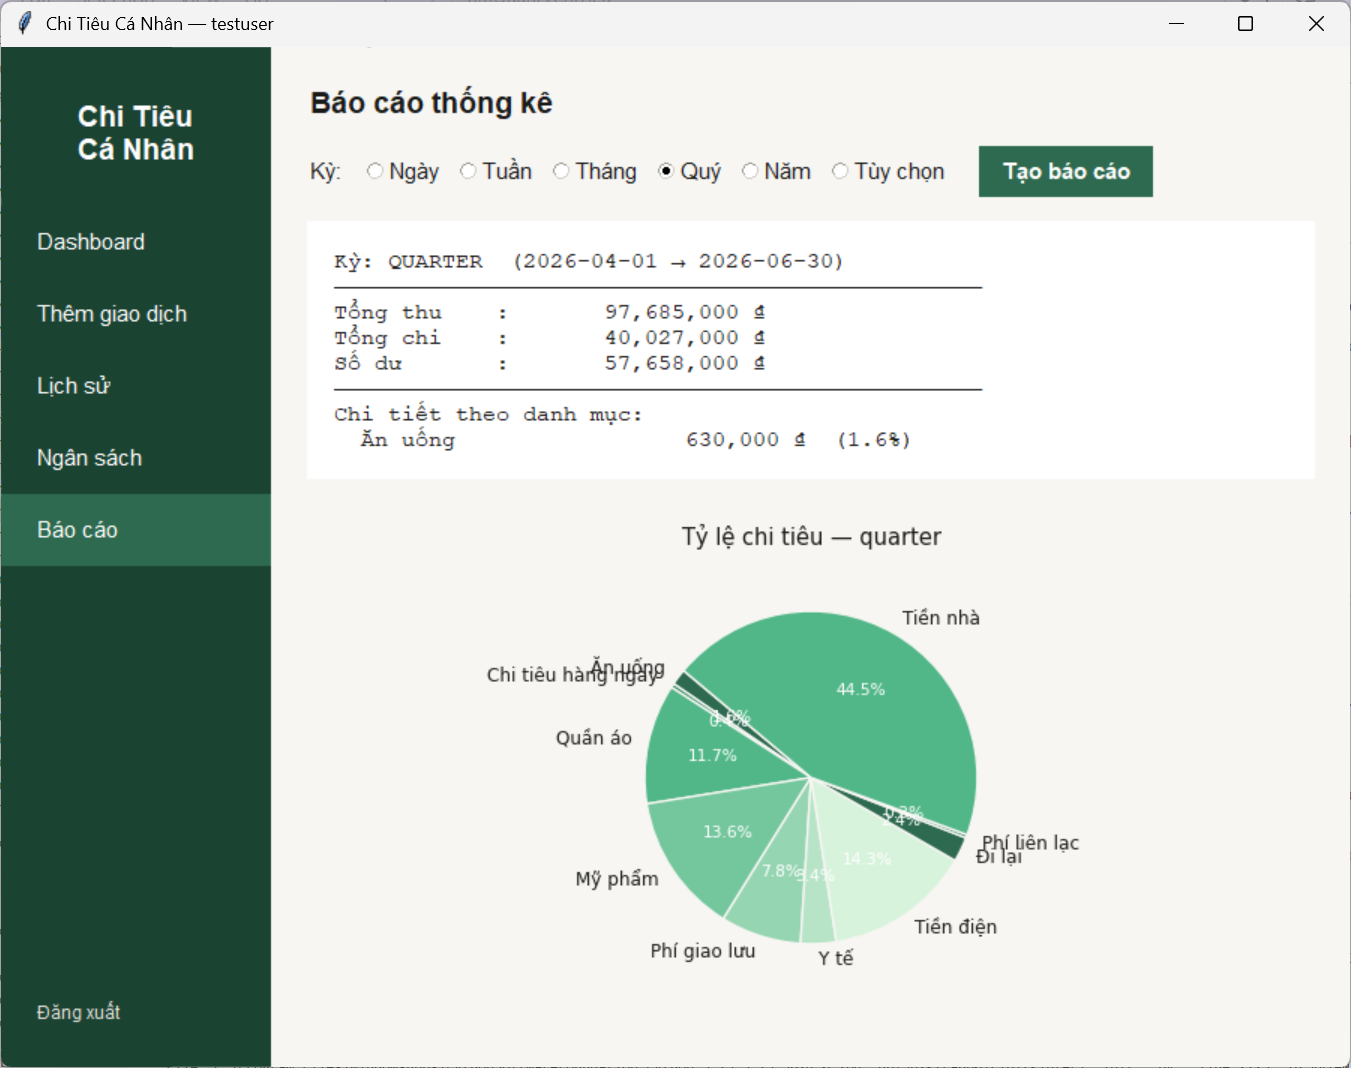
\includegraphics[width=0.85\textwidth]{OUT_TC19.png}
    \par\vspace{0.2cm} 
    \small\textbf{TC-019}

    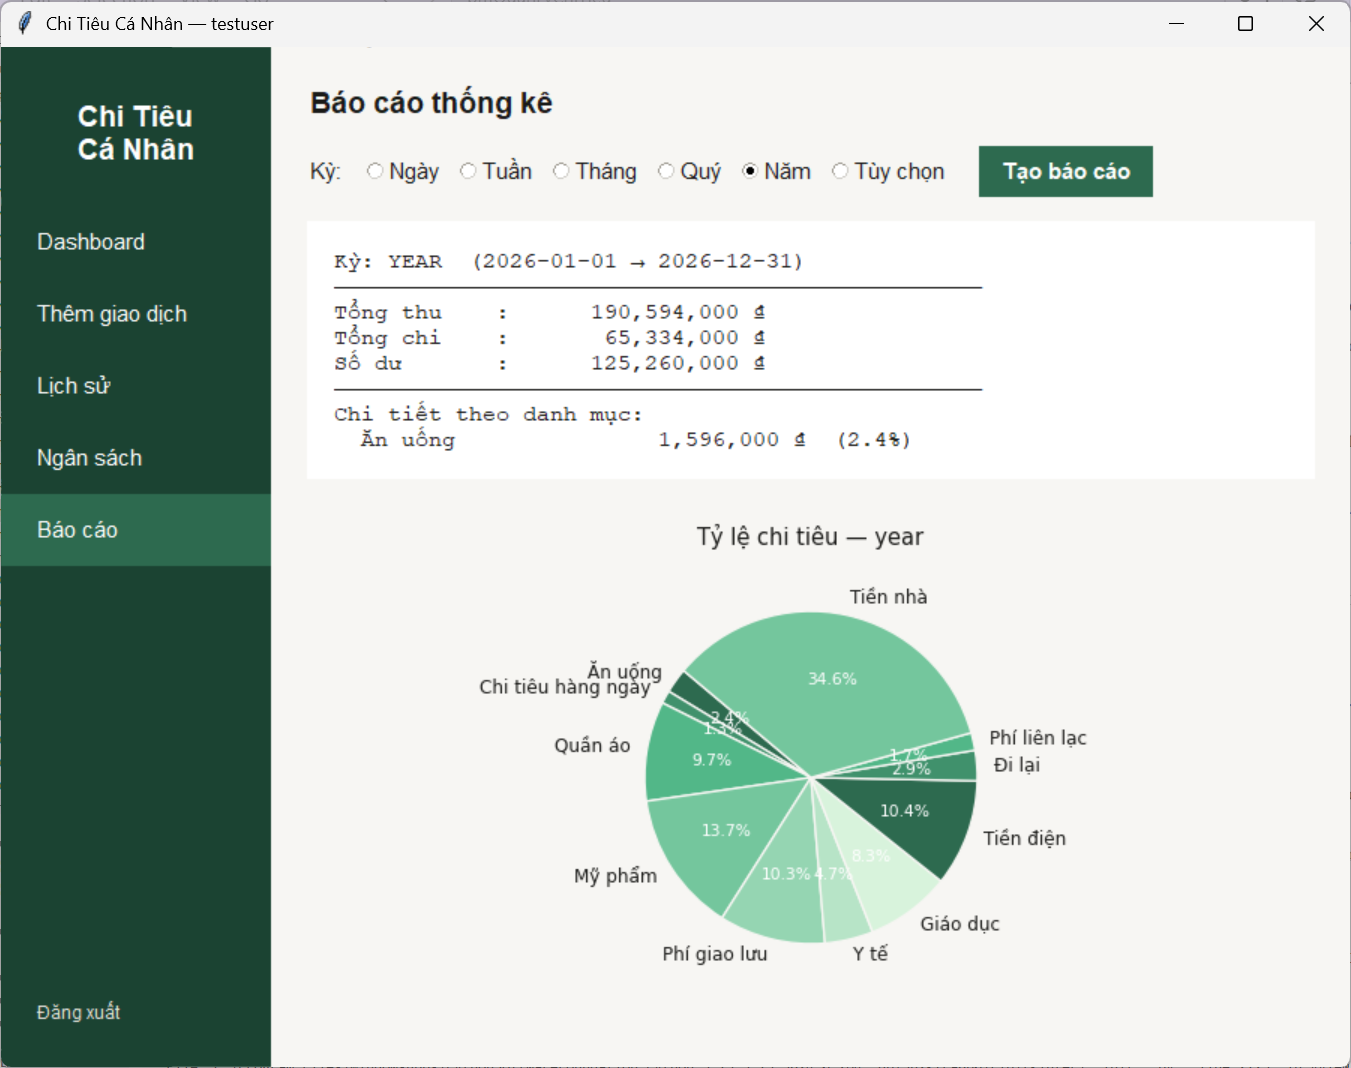
\includegraphics[width=0.85\textwidth]{OUT_TC20.png}
    \par\vspace{0.3cm} 
    \small\textbf{TC-020}

    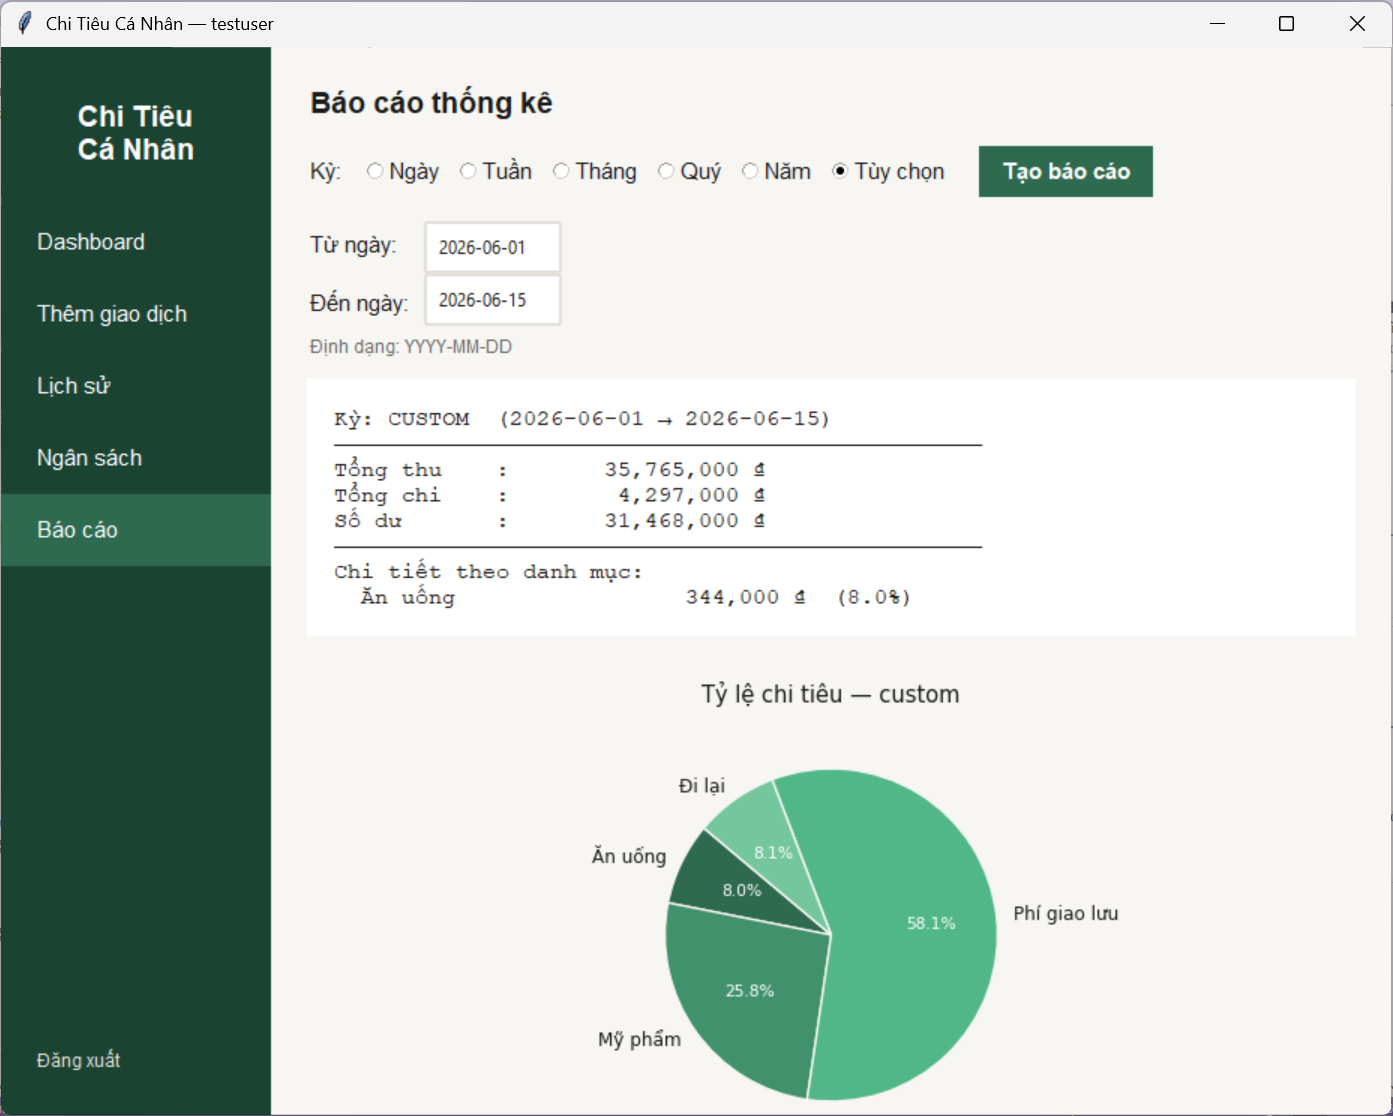
\includegraphics[width=0.85\textwidth]{OUT_TC21.png}
    \par\vspace{0.3cm} 

    \small\textbf{TC-021}
    \vspace{0.3cm}
\end{center}

\newpage
\section{Các kĩ thuật sử dụng}
Hệ thống được cài đặt bằng Python theo hình mẫu lập trình hướng đối tượng, sử dụng cấu trúc dữ liệu tự cài đặt LinkedList thay vì các cấu trúc có sẵn, lưu trữ dữ liệu dưới dạng file JSON, và xây dựng giao diện đồ hoạ bằng Tkinter kết hợp Matplotlib.
\subsection{Kỹ thuật đặt tên và chú thích}
Đặt tên là kỹ thuật nền tảng trong lập trình có cấu trúc, quyết định trực tiếp đến khả năng đọc hiểu và bảo trì của mã nguồn. Theo nguyên tắc kỹ thuật lập trình kinh điển Clean Code của Robert C. Martin, một tên gọi tốt cần thoả mãn:

\begin{itemize}
    \item Có nghĩa và thể hiện đúng mục đích
    \item Nhất quán về quy ước trên toàn dự án
    \item Phân biệt rõ vai trò qua quy ước
    \item Độ dài tương xứng với phạm vi sử dụng
\end{itemize}

Chú thích được dùng để bổ sung ngữ cảnh, lý do thiết kế, hoặc cảnh báo tác dụng phụ mà tên hàm không thể truyền tải hết.

Quy ước đặt tên áp dụng trong hệ thống được mô tả như trong bảng dưới
\begin{table}[h!]
    \centering
    \renewcommand{\arraystretch}{1.4}
    \begin{tabular}{|p{3.5cm}|p{4.5cm}|p{7cm}|}
        \hline
        \textbf{Thành phần} & \textbf{Quy ước} & \textbf{Ví dụ trong mã nguồn} \\
        \hline
        Tên lớp (Class) & PascalCase, danh từ & TransactionService, BudgetRepository, LinkedList \\
        \hline
        Tên hàm/method & snake\_case, động từ & add\_transaction(), get\_month\_status(), \_validate\_date() \\
        \hline
        Tên biến & snake\_case, danh từ & total\_income, budget\_limit, category\_id \\
        \hline
        Hằng số & UPPER\_SNAKE\_CASE & DEFAULT\_EXPENSE\_CATEGORIES, ALLOWED\_TLDS \\
        \hline
        Phương thức private & tiền tố dấu gạch dưới \_ & \_validate\_month(), \_check\_budget(), \_next\_id() \\
        \hline
        Tên file module & snake\_case, số ít & transaction\_service.py, budget\_repository (trong file) \\
        \hline
    \end{tabular}
\end{table}

Ngoài ra, hệ thống sử dụng hai loại chú thích với mục đích khác nhau: docstring ở đầu các module, class, hàm và inline comment cho các đoạn chương . Ví dụ, trong hàm \texttt{validate and normalize amount} sử dụng cả 2 loại chú thích này
\begin{lstlisting}[language=Python]
def _validate_and_normalize_amount(self, amount):
    """
    Xac thuc va chuan hoa so tien.
    - Chuyen doi thanh float
    - Kiem tra > 0
    - Lam tron 2 chu so thap phan
    Tra ve (is_valid: bool, amount_normalized: float, error_message: str)
    """
    if not amount:
        return False, None, "So tien khong duoc de trong."
    
    try:
        # Chuyen doi thanh float (da duoc chuan hoa tu UI)
        amount_float = float(amount)
    except (ValueError, TypeError):
        return False, None, "So tien khong hop le. Vui long nhap so."
    
    # Kiem tra > 0
    if amount_float <= 0:
        return False, None, "So tien phai lon hon 0."
    
    # Lam tron 2 chu so thap phan
    amount_normalized = round(amount_float, 2)
    
    return True, amount_normalized, ""
\end{lstlisting}
\subsection{Kỹ thuật sử dụng hàm}
Hàm, thủ tục hay chương trình con là đơn vị phân rã cơ bản của lập trình có cấu trúc, dựa trên nguyên lý chia để trị : một bài toán lớn được tách thành các bài toán con độc lập, mỗi bài toán con được giải quyết bởi một hàm có trách nhiệm duy nhất. Ví dụ, trong mã nguồn của hệ thống, chức năng \texttt{Thêm giao dịch} không được viết thành một hàm khổng lồ duy nhất, mà được phân rã thành chuỗi các hàm con, mỗi hàm đảm nhiệm đúng một bước:
\begin{lstlisting}[language=Python]
# transaction_service.py
def add_transaction(self, user_id, category_id, amount, type, note="", date=None):
    # Buoc 1: Xac thuc va chuan hoa so tien
    is_valid, amount_normalized, error_msg = self._validate_and_normalize_amount(amount)
    if not is_valid:
        raise ValueError(error_msg)

    if type not in ("income", "expense"):
        raise ValueError("Loai giao dich phai la 'income' hoac 'expense'.")

    # Buoc 2: Xac thuc ngay
    date_to_use = date or datetime.now().strftime("%Y-%m-%d")
    is_valid, error_msg = self._validate_date(date_to_use)
    if not is_valid:
        raise ValueError(error_msg)

    # Buoc 3: Tao va luu doi tuong
    tx = Transaction(id=0, user_id=user_id, category_id=category_id,
                      amount=amount_normalized, type=type, note=note, date=date_to_use)
    saved_tx = self.tx_repo.add(tx)

    # Buoc 4: Kiem tra ngan sach (chi voi khoan chi)
    alert = None
    if type == "expense":
        alert = self._check_budget(user_id, category_id, saved_tx.date)
    return saved_tx, alert
\end{lstlisting}
\subsection{Kỹ thuật quản lý và xử lý dữ liệu}

Hệ thống sử dụng Danh sách liên kết đơn tự cài đặt trong tầng \texttt{models} làm cấu trúc lưu trữ dữ liệu chính trong bộ nhớ RAM thay vì mảng hay list có sẵn của Python. Lớp này cung cấp các thao tác cơ bản như append, get, remove, find và filter. Toàn bộ dữ liệu load từ JSON lên đều được chuyển thành đối tượng và lưu trong LinkedList. Các lớp Repository sẽ sử dụng hàm filter() để duyệt tuần tự và trích xuất dữ liệu thỏa mãn điều kiện thành một danh sách mới.

Ngoài ra, dữ liệu của hệ thống được lưu trữ bền vững cục bộ dưới định dạng văn bản JSON. Cụ thể, trong thư mục \texttt{data}, dữ liệu được lưu trữ, thực hiện ghi và lấy thông tin ở các files \texttt{budgets.json, categories.json, reports.json, transactrions.json, user.json}. Hai quá trình chính trong việc lưu trữ là tuần tự hóa bằng \texttt{json.dump()} và giải tuần tự hóa bằng \texttt{json.load()}. Mỗi lớp model tự định nghĩa phương thức \texttt{to\_dict()} và \texttt{from\_dict()} để thực hiện chuyển đổi này. Đối với mô hình phức tạp như Report, các thuộc tính chứa LinkedList được gọi hàm \texttt{to\_list()} chuyển về dạng mảng thường để có thể ghi ra JSON. Hệ thống cũng áp dụng chiến lược lưu trữ write-through toàn phần, nghĩa là mỗi khi có một thao tác thay đổi dữ liệu, toàn bộ cấu trúc trong RAM sẽ được ghi đè xuống file JSON.
\subsection{Kỹ thuật trình bày mã}
Hệ thống sử dụng kiến trúc phân tầng chia chương trình thành các tầng có trách nhiệm riêng biệt, tầng trên chỉ gọi xuống tầng dưới và không có chiều ngược lại.
\begin{figure}[H]
    \centering
    \renewcommand{\arraystretch}{1.3} 
    \begin{tabular}{@{} l l @{}} 
    \texttt{|-\/-\/- models} & \\
    \texttt{| \ \ |-\/-\/- linked\_list.py} & \\
    \texttt{| \ \ |-\/-\/- models.py} & \\
    \texttt{|-\/-\/- repositories} &  \\
    \texttt{| \ \ |-\/-\/- base\_repository.py} & \\
    \texttt{| \ \ |-\/-\/- repositories.py} & \\
    \texttt{|-\/-\/- services} &  \\
    \texttt{| \ \ |-\/-\/- budget\_service.py} & \\
    \texttt{| \ \ |-\/-\/- report\_service.py} & \\
    \texttt{| \ \ |-\/-\/- transaction\_service.py} & \\
    \texttt{| \ \ |-\/-\/- user\_service.py} & \\
    \texttt{|-\/-\/- ui} &  \\
    \texttt{| \ \ |-\/-\/- budget\_report\_frame.py} & \\
    \texttt{| \ \ |-\/-\/- dashboard\_frame.py} & \\
    \texttt{| \ \ |-\/-\/- login\_frame.py} & \\
    \texttt{| \ \ |-\/-\/- theme.py} & \\
    \texttt{| \ \ |-\/-\/- transaction\_frame.py} & \\
    \texttt{|-\/-\/- main.py} &  \\
    \end{tabular}
\end{figure}
Theo đó, sự phụ thuộc trong toàn bộ mã nguồn chỉ chạy theo một chiều: ui → services → repositoreies → models. Nhờ đó, mỗi tầng có thể được đọc, kiểm thử hoặc thay đổi mà ít ảnh hưởng tới các tầng còn lại.

\newpage
\section{Phụ lục hàm main}
\subsection{Mã nguồn hàm main}
\begin{lstlisting}[language=Python]
if __name__ == "__main__":
    app = App()
    app.mainloop()
\end{lstlisting}
\subsection{Phương thức khởi tạo}
\begin{lstlisting}[language=Python, escapeinside={(*}{*)}]
class App(tk.Tk):
    def __init__(self):
        super().__init__()
        self.title("(*Quản Lý Chi Tiêu Cá Nhân*)")
        self.geometry("900x680")
        self.minsize(800, 600)
        self.configure(bg=COLORS["bg"])
        apply_theme(self)

        self.current_user = None
        self._show_login()
\end{lstlisting}
\subsection{Các phương thức xử lý và điều hướng giao diện}
\subsubsection{Xóa giao diện hiện tại}
\begin{lstlisting}[language=Python]
    def _clear(self):
        for widget in self.winfo_children():
            widget.destroy()
\end{lstlisting}
\subsubsection{Xử lý đăng nhập}
\begin{lstlisting}[language=Python, escapeinside={(*}{*)}]
    def _show_login(self):
        self._clear()
        LoginFrame(self, on_login_success=self._on_login).pack(
            fill="both", expand=True)

    def _on_login(self, user):
        self.current_user = user
        self.title(f"(*Chi Tiêu Cá Nhân — *){user.name}")
        self._show_main()
\end{lstlisting}
\subsubsection{Xây dựng giao diện chính}
\begin{lstlisting}[language=Python, escapeinside={(*}{*)}]
    def _show_main(self):
        self._clear()

        # --- Sidebar ----------------------------------
        sidebar = tk.Frame(self, bg=COLORS["primary_dark"], width=180)
        sidebar.pack(side="left", fill="y")
        sidebar.pack_propagate(False)

        tk.Label(sidebar, text="(*Chi Tiêu*)\n(*Cá Nhân*)",
                 font=FONTS["subhead"], fg="#FFFFFF",
                 bg=COLORS["primary_dark"],
                 justify="center").pack(pady=(32, 24))

        menu_items = [
            ("Dashboard",       "dashboard"),
            ("(*Thêm giao dịch*)",  "add_transaction"),
            ("(*Lịch sử*)",        "history"),
            ("(*Ngân sách*)",      "budget"),
            ("(*Báo cáo*)",        "report"),
        ]
        self._nav_btns = {}
        for label, key in menu_items:
            btn = tk.Button(
                sidebar, text=label,
                font=FONTS["body"],
                fg="#FFFFFF", bg=COLORS["primary_dark"],
                activeforeground="#FFFFFF",
                activebackground=COLORS["primary"],
                relief="flat", anchor="w",
                padx=20, pady=10,
                cursor="hand2",
                command=lambda k=key: self._navigate(k),
            )
            btn.pack(fill="x")
            self._nav_btns[key] = btn

        # (*Nút đăng xuất*)
        tk.Button(sidebar, text="(*Đăng xuất*)",
                  font=FONTS["small"],
                  fg=COLORS["border"], bg=COLORS["primary_dark"],
                  activeforeground="#FFFFFF",
                  activebackground=COLORS["danger"],
                  relief="flat", anchor="w",
                  padx=20, pady=8,
                  cursor="hand2",
                  command=self._logout).pack(side="bottom", fill="x",
                                             pady=(0, 16))

        # --- Content area -----------------------------
        self.content = tk.Frame(self, bg=COLORS["bg"])
        self.content.pack(side="right", fill="both", expand=True)

        self._navigate("dashboard")
\end{lstlisting}
\subsubsection{Điều hướng chức năng}
\begin{lstlisting}[language=Python, escapeinside={(*}{*)}]
    def _navigate(self, screen):
        # (*Highlight nút active*)
        for key, btn in self._nav_btns.items():
            btn.config(bg=COLORS["primary"] if key == screen
                       else COLORS["primary_dark"])

        # (*Xoá nội dung cũ*)
        for w in self.content.winfo_children():
            w.destroy()

        user = self.current_user

        if screen == "dashboard":
            frame = DashboardFrame(self.content, user,
                                   on_navigate=self._navigate)
        elif screen == "add_transaction":
            frame = AddTransactionFrame(
                self.content, user,
                on_save=lambda: self._navigate("dashboard"))
        elif screen == "history":
            frame = TransactionListFrame(self.content, user)
        elif screen == "budget":
            frame = BudgetFrame(self.content, user)
        elif screen == "report":
            frame = ReportFrame(self.content, user)
        else:
            return

        frame.pack(fill="both", expand=True)
\end{lstlisting}
\subsubsection{Xử lý đăng xuất}
\noindent % Thêm cái này để hộp code không bị lùi vào một khoảng thụt đầu dòng
\begin{minipage}{\linewidth}
\begin{lstlisting}[language=Python, escapeinside={(*}{*)}]
    def _logout(self):
        self.current_user = None
        self.title("(*Quản Lý Chi Tiêu Cá Nhân*)")
        self._show_login()
\end{lstlisting}
\end{minipage}

\newpage
\section{Phân công công việc}
\begin{table}[htbp]
\centering
% Định nghĩa độ rộng các cột: STT (căn giữa), Thành viên (căn trái), Nội dung (độ rộng cố định 6.5cm), Đánh giá (căn giữa)
\begin{tabular}{|c|p{4cm}|p{6.5cm}|c|}
\hline
\textbf{STT} & \textbf{Thành viên} & \textbf{Nội dung công việc} & \textbf{Đánh giá} \\ \hline
1 & Phạm Thị Ninh & 
- Phân tích bài toán \newline 
- Thiết kế chương trình \newline 
- Phụ lục hàm main & A \\ \hline
2 & Hứa Ngọc Khánh & 
- Viết mã nguồn\newline
- Gỡ lỗi và kiểm thử \newline 
- Các kĩ thuật sử dụng & A \\ \hline
\end{tabular}
\caption{Bảng phân công nhiệm vụ chi tiết của các thành viên}
\label{tab:phan_cong_cong_viec}
\end{table}

\newpage
\section{Phụ lục mã nguồn}
Mã nguồn chi tiết của dự án được công khai trên GitHub tại địa chỉ: \url{https://github.com/khanh-hua-kkk/pmQuanLyChiTieu.git}
\end{document}